%!Mode:: "TeX:UTF-8"
\documentclass[a4paper,11pt,UTF8]{ctexart}

\usepackage{indentfirst} %缩进
\usepackage{xeCJK}    %使用系统字体
\usepackage{fancyhdr} %自定义页眉页脚
\pagestyle{empty}                   %不设置页眉页脚
\usepackage{amsmath, amsthm, amssymb, amsfonts} %数学公式
\usepackage[a4paper,left=3cm,right=3cm,top=3cm,bottom=3cm]{geometry}
%\usepackage[tmargin=1in,bmargin=1in,lmargin=1.25in,rmargin=1.25in]{geometry}.
\usepackage{booktabs} %插入表格
\usepackage[section]{placeins} %避免浮动
\usepackage{listings} %插入代码
\usepackage{ctex}     %中文宏包
\usepackage[svgnames, table]{xcolor} %彩色表格
\usepackage{algorithm}          %伪代码
\usepackage{algorithmicx}
\usepackage{algpseudocode}
\usepackage{algorithm,algpseudocode,float}
\usepackage{lipsum}
\usepackage{enumitem}           %调整列举环境
\usepackage{url}
\usepackage{fontspec,xunicode}
\usepackage{subfigure}
\usepackage{parskip}      %m行n列图片排版方法
\defaultfontfeatures{Mapping=tex-text} %如果没有它,会有一些 tex 特殊字符无法正常使用,比如连字符。

\usepackage{graphicx}
\graphicspath{{imgs/}}

%%%%%%%%%%%%%%%%%%%%%%%%%%%%%%%%%%%%%%%%%%%%%%%%%%%%%%%%%%%%%%%%
% 缩进及行间距
%%%%%%%%%%%%%%%%%%%%%%%%%%%%%%%%%%%%%%%%%%%%%%%%%%%%%%%%%%%%%%%%
\setlength{\parindent}{22pt} %重新定义缩进长度
\setlength{\baselineskip}{20pt}  %定义行间距
%\renewcommand{\baselinestretch}{1.1} %定义行间距

%%%%%%%%%%%%%%%%%%%%%%%%%%%%%%%%%%%%%%%%%%%%%%%%%%%%%%%%%%%%%%%%
% 列表设置
%%%%%%%%%%%%%%%%%%%%%%%%%%%%%%%%%%%%%%%%%%%%%%%%%%%%%%%%%%%%%%%%
\setenumerate{fullwidth,itemindent=\parindent,listparindent=\parindent,itemsep=0ex,partopsep=0pt,parsep=0ex}
\setenumerate[2]{label=\alph*),leftmargin=1.5em}  %二级item设置
\setitemize{itemindent=38pt,leftmargin=0pt,itemsep=-0.4ex,listparindent=26pt,partopsep=0pt,parsep=0.5ex,topsep=-0.25ex}
\setdescription{itemindent=38pt,leftmargin=0pt,itemsep=-0.4ex,listparindent=26pt,partopsep=0pt,parsep=0.5ex,topsep=-0.25ex}

%%%%%%%%%%%%%%%%%%%%%%%%%%%%%%%%%%%%%%%%%%%%%%%%%%%%%%%%%%%%%%%%
% 图的标题行间距设置
%%%%%%%%%%%%%%%%%%%%%%%%%%%%%%%%%%%%%%%%%%%%%%%%%%%%%%%%%%%%%%%%
\newcommand{\bottomcaption}{%
\setlength{\abovecaptionskip}{6pt}%
\setlength{\belowcaptionskip}{6pt}%
\caption}


%%%%%%%%%%%%%%%%%%%%%%%%%%%%%%%%%%%%%%%%%%%%%%%%%%%%%%%%%%%%%%%%
% 字体定义
%%%%%%%%%%%%%%%%%%%%%%%%%%%%%%%%%%%%%%%%%%%%%%%%%%%%%%%%%%%%%%%%
\setmainfont{Times New Roman}  %默认英文字体.serif是有衬线字体sans serif无衬线字体
\setmonofont{FiraCode-Retina.ttf}
\setCJKmainfont[ItalicFont={楷体}, BoldFont={黑体}]{宋体}%衬线字体 缺省中文字体为
\setCJKsansfont{黑体}
\punctstyle{hangmobanjiao}
%-----------------------xeCJK下设置中文字体------------------------------%
\setCJKfamilyfont{song}{SimSun}                             %宋体 song
\newcommand{\song}{\CJKfamily{song}}
\setCJKfamilyfont{fs}{FangSong}                      %仿宋  fs
\newcommand{\fs}{\CJKfamily{fs}}
\setCJKfamilyfont{ktgb}{KaiTi}                      %楷体2312 ktgb
\newcommand{\ktgb}{\CJKfamily{ktgb}}
\setCJKfamilyfont{yh}{Microsoft YaHei}                    %微软雅黑 yh
\newcommand{\yh}{\CJKfamily{yh}}
\setCJKfamilyfont{hei}{SimHei}                              %黑体  hei
\newcommand{\hei}{\CJKfamily{hei}}
\setCJKfamilyfont{hwxk}{STXingkai}                                %华文行楷  hwxk
\newcommand{\hwxk}{\CJKfamily{hwxk}}
%------------------------------设置字体大小------------------------%
\newcommand{\shiyanbaogao}{\fontsize{36pt}{\baselineskip}\selectfont}
\newcommand{\chuhao}{\fontsize{42pt}{\baselineskip}\selectfont}     %初号
\newcommand{\xiaochuhao}{\fontsize{36pt}{\baselineskip}\selectfont} %小初号
\newcommand{\yihao}{\fontsize{28pt}{\baselineskip}\selectfont}      %一号
\newcommand{\erhao}{\fontsize{21pt}{\baselineskip}\selectfont}      %二号
\newcommand{\xiaoerhao}{\fontsize{18pt}{\baselineskip}\selectfont}  %小二号
\newcommand{\sanhao}{\fontsize{15.75pt}{\baselineskip}\selectfont}  %三号
\newcommand{\sihao}{\fontsize{14pt}{\baselineskip}\selectfont}       %四号
\newcommand{\xiaosihao}{\fontsize{12pt}{\baselineskip}\selectfont}  %小四号
\newcommand{\wuhao}{\fontsize{10.5pt}{\baselineskip}\selectfont}    %五号
\newcommand{\xiaowuhao}{\fontsize{9pt}{\baselineskip}\selectfont}   %小五号
\newcommand{\liuhao}{\fontsize{7.875pt}{\baselineskip}\selectfont}  %六号
\newcommand{\qihao}{\fontsize{5.25pt}{\baselineskip}\selectfont}    %七号

%%%%%%%%%%%%%%%%%%%%%%%%%%%%%%%%%%%%%%%%%%%%%%%%%%%%%%%%%%%%%%%%
% 图题字体大小相同
%%%%%%%%%%%%%%%%%%%%%%%%%%%%%%%%%%%%%%%%%%%%%%%%%%%%%%%%%%%%%%%%
\usepackage{caption}
\captionsetup{font={footnotesize}}   % footnotesize = 9pt
\captionsetup[lstlisting]{font={footnotesize}}

%%%%%%%%%%%%%%%%%%%%%%%%%%%%%%%%%%%%%%%%%%%%%%%%%%%%%%%%%%%%%%%%
% 重定义枚举编号为 1),2)...
%%%%%%%%%%%%%%%%%%%%%%%%%%%%%%%%%%%%%%%%%%%%%%%%%%%%%%%%%%%%%%%%
\renewcommand{\labelenumi}{\theenumi)}


%%%%%%%%%%%%%%%%%%%%%%%%%%%%%%%%%%%%%%%%%%%%%%%%%%%%%%%%%%%%%%%%
% 重定义section标题
%%%%%%%%%%%%%%%%%%%%%%%%%%%%%%%%%%%%%%%%%%%%%%%%%%%%%%%%%%%%%%%%
\CTEXsetup[format={\sihao\CJKfamily{zhhei}\zihao{4}},number={\chinese{section}},name={,、~},aftername={},indent={0pt},beforeskip={6pt},afterskip={6pt},format+={\flushleft}]{section}
\CTEXsetup[format={\Large\bfseries\CJKfamily{zhkai}\zihao{5}},name={(,)},number={\chinese{subsection}},aftername={},indent={22pt},beforeskip={14pt},afterskip={2pt}]{subsection}
\CTEXsetup[number={\chinese{section}},name={附录, ~~ }]{appendix}



%%%%%%%%%%%%%%%%%%%%%%%%%%%%%%%%%%%%%%%%%%%%%%%%%%%%%%%%%%%%%%%%
% 标题名称中文化
%%%%%%%%%%%%%%%%%%%%%%%%%%%%%%%%%%%%%%%%%%%%%%%%%%%%%%%%%%%%%%%%
\renewcommand\figurename{\hei 图}
\renewcommand\tablename{\hei 表}
\renewcommand\lstlistingname{\hei 代码}
\renewcommand{\algorithmicrequire}{\textbf{输入:}}
\renewcommand{\algorithmicensure}{\textbf{输出:}}
\newtheorem{define}{定义}

%%%%%%%%%%%%%%%%%%%%%%%%%%%%%%%%%%%%%%%%%%%%%%%%%%%%%%%%%%%%%%%%
% 代码设置
%%%%%%%%%%%%%%%%%%%%%%%%%%%%%%%%%%%%%%%%%%%%%%%%%%%%%%%%%%%%%%%%
\lstset{
 columns=fixed,
 numbers=left,                                        % 在左侧显示行号
 numberstyle=\tiny\color{gray},                       % 设定行号格式
 frame=single,                                      % 单线背景边框
%  frame=none,                                          % 不显示背景边框
 breaklines=true,                                     % 设定LaTeX对过长的代码行进行自动换行
 tabsize=4,                                           % 把tab扩展为4个空格,默认是8个太长
 keywordstyle=\color[RGB]{40,40,255},                 % 设定关键字颜色
 numberstyle=\footnotesize\color{darkgray}\ttfamily,
 commentstyle=\it\color[RGB]{0,96,96}\ttfamily,       % 设置代码注释的格式
 stringstyle=\rmfamily\slshape\color[RGB]{128,0,0},   % 设置字符串格式
 showstringspaces=false,                              % 不显示字符串中的空格
 language=c++,                                        % 设置语言
 basicstyle=\linespread{0.7}\xiaowuhao\ttfamily,                      % 字体字号
 morekeywords={alignas,continute,friend,register,true,alignof,decltype,goto,
 reinterpret_cast,try,asm,defult,if,return,typedef,auto,delete,inline,short,
 typeid,bool,do,int,signed,typename,break,double,long,sizeof,union,case,
 dynamic_cast,mutable,static,unsigned,catch,else,namespace,static_assert,using,
 char,enum,new,static_cast,virtual,char16_t,char32_t,explict,noexcept,struct,
 void,export,nullptr,switch,volatile,class,extern,operator,template,wchar_t,
 const,false,private,this,while,constexpr,float,protected,thread_local,
 const_cast,for,public,throw,std},
 xleftmargin=2em,
 xrightmargin=2em,
 aboveskip=1em
 %lineskip=10pt,
 %baselinestretch=1,
}

%%%%%%%%%%%%%%%%%%%%%%%%%%%%%%%%%%%%%%%%%%%%%%%%%%%%%%%%%%%%%%%%
% 伪代码分页
%%%%%%%%%%%%%%%%%%%%%%%%%%%%%%%%%%%%%%%%%%%%%%%%%%%%%%%%%%%%%%%%
\makeatletter
\renewcommand{\ALG@name}{算法}
\newenvironment{breakablealgorithm}
  {% \begin{breakablealgorithm}
   \begin{center}
     \refstepcounter{algorithm}% New algorithm
     \hrule height.8pt depth0pt \kern2pt% \@fs@pre for \@fs@ruled
     \renewcommand{\caption}[2][\relax]{% Make a new \caption
       {\raggedright\textbf{\ALG@name~\thealgorithm} ##2\par}%
       \ifx\relax##1\relax % #1 is \relax
         \addcontentsline{loa}{algorithm}{\protect\numberline{\thealgorithm}##2}%
       \else % #1 is not \relax
         \addcontentsline{loa}{algorithm}{\protect\numberline{\thealgorithm}##1}%
       \fi
       \kern2pt\hrule\kern2pt
     }
  }{% \end{breakablealgorithm}
     \kern2pt\hrule\relax% \@fs@post for \@fs@ruled
   \end{center}
  }
\makeatother



\begin{document}
\xiaosihao\song

\begin{titlepage}
\center{\yihao{\hwxk{南京航空航天大学}}}
\vspace{6cm}
\center{\shiyanbaogao{\ktgb{课~程~设~计}}}
\vspace{4cm}

\begin{center}
\begin{large}
\begin{tabular}{rc}
  \xiaoerhao{\hei{课\qquad 程}}& \hspace{1.7cm}\xiaoerhao{\hei{数据结构\hspace{1.7cm}}} \\
  \cline{2-2}\\
  \xiaoerhao{\hei{班\qquad 级}}& \hspace{1.7cm}\xiaoerhao{\hei{1819001\hspace{1.7cm}}} \\
  \cline{2-2}\\
  \xiaoerhao{\hei{学\qquad 号}}& \hspace{1.7cm}\xiaoerhao{\hei{161940233\hspace{1.7cm}}} \\
  \cline{2-2}\\
  \xiaoerhao{\hei{姓\qquad 名}}& \xiaoerhao{\hei{颜~宇~明}}\\
  \cline{2-2}\\
  \xiaoerhao{\hei{指导教师}}& \xiaoerhao{\hei{秦~小~麟}}\\
  \cline{2-2}
\end{tabular}
\end{large}
\end{center}
\vfill \hfill
\end{titlepage}
\clearpage


% \centerline{\\[10pt]\erhao{\fs{目~~录}}}
\tableofcontents
\newpage
\section{区块链}
\subsection{数据结构}
链表
\subsection{算法设计思想}
将区块设计成链表节点,每增加一个节点,计算校验码都要结合之前所有的节点的信息。
\subsection{源程序}
\begin{lstlisting}[caption=Linked\_list.h,captionpos=b]
#ifndef LINKED_LIST_H
#define LINKED_LIST_H
class ADT_list{
public:
    typedef struct node
    {
        int number;
        char information[100];
        int Checkcode;
        node *next;
    } node;
    node *head;
    int length = -1;

    void InitLIst();
    void DestoryList();
    void ClearList();
    bool ListEmpty();
    int ListLength();
    node* GetElem(int);
    int LocateElem(int);
    int PriorElem(int);
    int NextElem(int);
    void ListTraverse();
    void CreateList(char*, int);
    int CheckList();
    void SetStr(int, const char*);
    void InsertElem(char*);
    int GetCheckcode();
    void DeleteElem(int index);
    void Reverse();
};
#endif
\end{lstlisting}

\begin{lstlisting}[caption=Linked\_list.cpp,captionpos=b]
  #include <malloc.h>
  #include <stdio.h>
  #include <string.h>
  #include "Linked_list.h"

  void ADT_list::InitLIst(){
      node *tmp = (node *)malloc(sizeof(node));
      length = 0;
      head = tmp;
      tmp->next = NULL;
  }

  void ADT_list::DestoryList(){
      node *p, *temp;
      p = head;
      while (p != NULL){
          temp = p;
          p = p->next;
          free(temp);
      }
      length = -1;
  }

  void ADT_list::ClearList(){
      node *p, *temp;
      p = head->next;
      while (p != NULL){
          temp = p;
          p = p->next;
          free(temp);
      }
      length = 0;
      head->next = NULL;
  }

  bool ADT_list::ListEmpty(){
      if (length < 1) return true;
      return false;
  }

  int ADT_list::ListLength(){
      return length;
  }

  ADT_list::node* ADT_list::GetElem(int index){
      node *p;
      int i = 0;
      p = head->next;
      while (p != NULL){
          if (index == ++i)
              return p;
          p = p->next;
      }
      return NULL;
  }

  int ADT_list::LocateElem(int num){
      node *p;
      p = head->next;
      int index = 0;
      while (p != NULL){
          if (p->number == num)
              return index;
          p = p->next;
          index++;
      }
      return -1;
  }

  int ADT_list::PriorElem(int cur_num){
      node *p, *temp;
      p = head->next;
      while (p != NULL){
          temp = p;
          p = p->next;
          if (p != NULL && p->number == cur_num)
              return temp->number;
      }
      return 0;
  }

  int ADT_list::NextElem(int cur_num){
      node *p, *temp;
      p = head->next;
      while (p != NULL){
          temp = p;
          p = p->next;
          if (p != NULL && temp->number == cur_num)
              return p->number;
      }
      return 0;
  }

  void ADT_list::ListTraverse(){
      node *p;
      p = head->next;
      puts("Block Chain Output:");
      while (p != NULL){
          printf("%d %s %d\n", p->number, p->information, p->Checkcode);
          p = p->next;
      }
      printf("\n");
  }

  void ADT_list::CreateList(char* str, int check){
      node *p = head;
      while (p->next != NULL) p = p->next;
      node *tmp = (node *)malloc(sizeof(node));
      p->next = tmp;
      tmp->next = NULL;
      tmp->number = length;
      strcpy(tmp->information, str);
      length++;
      tmp->Checkcode = check;
  }

  int ADT_list::CheckList(){
      node* p = head->next, *tmp = p;
      if (!p) return 1;
      while(p) {
          int sum = 0;
          for (int i = 0; i < strlen(p->information); i++)
              sum += p->information[i];
          if (p->number) {
              node *temp = head;
              sum += p->number;
              while (temp->next != p) temp = temp->next;
              sum += temp->Checkcode;
          }
          // printf("%d %d %d\n", sum % 113, p->Checkcode, p->number);
          if (sum % 113 != p->Checkcode) return p->number + 100;
          p = p->next;
      }
      return 1;
  }

  void ADT_list::SetStr(int index, const char* str){
      node *p;
      int i = 0;
      p = head->next;
      while (p && index != i++) p = p->next;
      strcpy(p->information, str);
      while(p) {
          int sum = 0;
          for (int i = 0; i < strlen(p->information); i++)
              sum += p->information[i];
          if (p->number) {
              node *temp = head;
              sum += p->number;
              while (temp->next != p) temp = temp->next;
              sum += temp->Checkcode;
          }
          // printf("%d %d %d\n", sum % 113, p->Checkcode, p->number);
          // if (sum % 113 != p->Checkcode) return p->number + 100;
          p->Checkcode = sum % 113;
          p = p->next;
      }
  }

  void ADT_list::InsertElem(char* str){
      node *p = head;
      while (p->next != NULL) p = p->next;
      node *tmp = (node *)malloc(sizeof(node));
      p->next = tmp;
      tmp->next = NULL;
      tmp->number = length;
      strcpy(tmp->information, str);
      length++;
      tmp->Checkcode = GetCheckcode();
  }
  int ADT_list::GetCheckcode(){
      node* p = head;
      while (p->next != NULL) p = p->next;
      int sum = 0;
      for (int i = 0; i < strlen(p->information); i++)
          sum += p->information[i];
      if (length > 1) {
          sum += p->number;
          p = head;
          while (p->next->next) p = p->next;
          sum += p->Checkcode;
      }
      return sum % 113;
  }
  void ADT_list::DeleteElem(int index){
      node *p, *temp;
      int i = 0;
      temp = head;
      p = head->next;
      length--;
      while (p != NULL){
          if (index != ++i) {
              temp = p;
              p = p->next;
              continue;
          }
          temp->next = p->next;
          free(p);
      }
  }

  void ADT_list::Reverse(){
      if (length < 1) return;
      node *p, *temp, *tmp = NULL;
      temp = p = head->next;
      while(temp != NULL){
          temp = p->next;
          p->next = tmp;
          tmp = p;
          p = temp;
      }
      head->next = tmp;
  }
  \end{lstlisting}
\begin{lstlisting}[caption=main.cpp,captionpos=b]
    #include <stdio.h>
    #include "Linked_list.h"
    char str[100];
    int num, check;
    int main(){
        ADT_list list;
        list.InitLIst();
        freopen("insertnode", "r", stdin);
        while (scanf("%s", &str) != EOF) list.InsertElem(str);
        list.ListTraverse();
        list.ClearList();
        freopen("CheckBlockChain", "r", stdin);
        while (scanf("%s%d", &str, &check) != EOF) list.CreateList(str, check);
        list.ListTraverse();
        (num = list.CheckList()) < 100 ? puts("Accept!") : printf("The %dth node Error!\n\n", num - 100);
        list.SetStr(1, "22");
        list.ListTraverse();

    }
\end{lstlisting}
\subsection{测试数据及其结果}
文件insertnode创建区块链输入:
\begin{lstlisting}
    3
    2
    1
\end{lstlisting}

文件CheckBlockChain创建一个错误的区块链:
\begin{lstlisting}
    3 51
    2 102
    1 4
\end{lstlisting}

main.cpp输出为:
\begin{lstlisting}
    Block Chain Output:
    0 3 51
    1 2 102
    2 1 40

    Block Chain Output:
    0 3 51
    1 2 102
    2 1 4

    The 2th node Error!

    Block Chain Output:
    0 3 51
    1 22 39
    2 1 90
\end{lstlisting}

由以上输出结果可知,题目要求所有完全达到了。

\subsection{时间复杂度}
$$
O(n)
$$
\subsection{改进方法}
算校验码不需要每次都把前面所有的节点都遍历一遍,可以直接用最后一个节点的校验码。

\section{迷宫问题}

\subsection{数据结构}
用栈来实现深度优先搜索
\subsection{算法设计思想}
先生成迷宫,设定起点,然后用栈实现的深度优先搜索来寻找迷宫的出口,迷宫保证路径唯一。
\subsection{源程序}

\begin{lstlisting}[caption=main.cpp,captionpos=b]
#include <stdio.h>
#include <stdlib.h>
#include "Sequence_Stack.h"
#include <fstream>
using namespace std;
int maze[100][100], n, visited[100][100];
int xx[] = {-1, 1, 0, 0};
int yy[] = {0, 0, -1, 1};
int endx, endy, flag;
ADT_Stack Stack;
string temp;
int main(){
    ifstream ReadFile("maze");
    while(getline(ReadFile, temp)) n++;

    Stack.InitStack();
    freopen("maze", "r", stdin);
    for (int i = 1; i <= n; i++)
    for (int j = 1; j <= n; j++)
        scanf("%d", &maze[i][j]);
    for (int i = n; i >= 1; i--)
        if (!maze[i][n]) endx = i, endy = n;

    Pos *point = new Pos;
    point->x = 2;
    point->y = 1;
    point->last = NULL;
    Stack.Push(*point);
    visited[point->x][point->y] = 1;
    while (Stack.rear) {
        Pos pp = Stack.Pop();
        Pos *p = new Pos;
        p->x = pp.x;
        p->y = pp.y;
        p->last = pp.last;
        visited[p->x][p->y] = 1;
        if (p->x == endx && p->y == endy) {
            point = p;
            while (point)
                maze[point->x][point->y] = 2, point = point->last;

            for (int i = 0; i <= n; i++) {
                for (int j = 0; j <= n; j++) {
                    if (maze[i][j] == 0)
                        printf("  ");
                    else if (maze[i][j] == 2)
                        printf("██");
                    else
                        printf("░░");
                }
                printf("\n");
            }
            return 0;
        }
        for (int i = 0; i < 4; i++)
            if (!maze[p->x + xx[i]][p->y + yy[i]] && !visited[p->x + xx[i]][p->y + yy[i]]) {
                point = new Pos;
                point->x = p->x + xx[i];
                point->y = p->y + yy[i];
                point->last = p;
                Stack.Push(*point);
            }
    }
}
\end{lstlisting}

\begin{lstlisting}[caption=MazeGeneration.cpp,captionpos=b]
#include<stdio.h>
#include<fstream>
#include<Windows.h>
#include<time.h>
#include<math.h>

//地图长度L,包括迷宫主体40,外侧的包围的墙体2,最外侧包围路径2(之后会解释)
#define L 44

//墙和路径的标识
#define WALL  0
#define ROUTE 1
using namespace std;
//控制迷宫的复杂度,数值越大复杂度越低,最小值为0
static int Rank = 0;
int startx = 2, starty = 1;

//生成迷宫
void CreateMaze(int **maze, int x, int y);

int main(void) {
    srand((unsigned)time(NULL));

    int **Maze = (int**)malloc(L * sizeof(int *));
    for (int i = 0; i < L; i++) {
        Maze[i] = (int*)calloc(L, sizeof(int));
    }

    //最外围层设为路径的原因,为了防止挖路时挖出边界,同时为了保护迷宫主体外的一圈墙体被挖穿
    for (int i = 0; i < L; i++){
        Maze[i][0] = ROUTE;
        Maze[0][i] = ROUTE;
        Maze[i][L - 1] = ROUTE;
        Maze[L - 1][i] = ROUTE;
    }

    //创造迷宫,(2,2)为起点
    CreateMaze(Maze, startx, starty + 1);

    //画迷宫的入口和出口
    Maze[2][1] = ROUTE;

    //由于算法随机性,出口有一定概率不在(L-3,L-2)处,此时需要寻找出口
    for (int i = L - 3; i >= 0; i--) {
        if (Maze[i][L - 3] == ROUTE) {
            Maze[i][L - 2] = ROUTE;
            break;
        }
    }

    //画迷宫
    for (int i = 0; i < L; i++) {
        for (int j = 0; j < L; j++) {
            if (Maze[i][j] == ROUTE) {
                printf("  ");
            }
            else {
                printf("██");
            }
        }
        printf("\n");
    }
    ofstream out("maze");
    if (out.is_open()){
        for (int i = 1; i < L - 1; i++) {
            for (int j = 1; j < L - 1; j++) {
                if (Maze[i][j] == ROUTE)
                    out << "0 ";
                else
                    out << "1 ";
            }
            out << "\n";
        }
    }

    for (int i = 0; i < L; i++) free(Maze[i]);
    free(Maze);

    return 0;
}

void CreateMaze(int **maze, int x, int y) {
    maze[x][y] = ROUTE;

    //确保四个方向随机
    int direction[4][2] = { { 1,0 },{ -1,0 },{ 0,1 },{ 0,-1 } };
    for (int i = 0; i < 4; i++) {
        int r = rand() % 4;
        int temp = direction[0][0];
        direction[0][0] = direction[r][0];
        direction[r][0] = temp;

        temp = direction[0][1];
        direction[0][1] = direction[r][1];
        direction[r][1] = temp;
    }

    //向四个方向开挖
    for (int i = 0; i < 4; i++) {
        int dx = x;
        int dy = y;

        //控制挖的距离,由Rank来调整大小
        int range = 1 + (Rank == 0 ? 0 : rand() % Rank);
        while (range>0) {
            dx += direction[i][0];
            dy += direction[i][1];

            //排除掉回头路
            if (maze[dx][dy] == ROUTE) {
                break;
            }

            //判断是否挖穿路径
            int count = 0;
            for (int j = dx - 1; j < dx + 2; j++) {
                for (int k = dy - 1; k < dy + 2; k++) {
                    //abs(j - dx) + abs(k - dy) == 1 确保只判断九宫格的四个特定位置
                    if (abs(j - dx) + abs(k - dy) == 1 && maze[j][k] == ROUTE) {
                        count++;
                    }
                }
            }

            if (count > 1) {
                break;
            }

            //确保不会挖穿时,前进
            --range;
            maze[dx][dy] = ROUTE;
        }

        //没有挖穿危险,以此为节点递归
        if (range <= 0) {
            CreateMaze(maze, dx, dy);
        }
    }
}
\end{lstlisting}


\begin{lstlisting}[caption=Sequence\_Stack.h,captionpos=b]
#ifndef SEQUENCE_Stack_H
#define SEQUENCE_Stack_H
typedef struct Pos
{
    int x;
    int y;
    Pos *last;
} Pos;
class ADT_Stack{
public:
    Pos Stack[9999];
    int rear = -1;
    void InitStack();
    void DestoryStack();
    void ClearStack();
    bool StackEmpty();
    int StackLength();
    Pos GetTop();
    void StackTraverse();
    void Push(Pos);
    Pos Pop();
    Pos operator [] (int);
    // int LocateElem(int num);
    // int PriorElem(int cur_num);
    // int NextElem(int cur_num);
    // int SetElem(int index, int num);
    // void InsertElem(int index, int num);
    // void DeleteElem(int index);
    // void Remove();
    // void Bubble_Sort();
    // void Select_sort();
    // ADT_Stack Union(ADT_Stack);
    // void Josephus(int);
};
#endif
\end{lstlisting}

\begin{lstlisting}[caption=Makefile, captionpos=b]
CC = g++

OUT1 = MazeGeneration.exe
OBJ1 = MazeGeneration.o

OUT2 = main.exe
OBJ2 = main.o Sequence_Stack.o

IN = main.cpp MazeGeneration.cpp Sequence_Stack.cpp

build: $(OUT1) $(OUT2)

run: $(OUT1) $(OUT2)
    @./$(OUT1);./$(OUT2)

clean:
    @rm -f *.o $(OUT1) $(OUT2)

$(OUT1): $(OBJ1)
    @$(CC) $(OBJ1) -o $(OUT1)

$(OUT2): $(OBJ2)
    @$(CC) $(OBJ2) -o $(OUT2)

$(OBJ): $(IN)
    @$(CC) -c $(IN)
\end{lstlisting}

\subsection{测试数据及其结果}

在项目目录下运行命令:
\begin{lstlisting}
    clear;make clean;make run
\end{lstlisting}

运行结果为:

\begin{figure}[htbp] % h为当前位置,!htb为忽略美学标准,htbp为浮动图形
    \centering
    \subfigure[自动生成的迷宫]{
        
\includegraphics[width=2.5in]{1.png}
        }
        \subfigure[基于DFS的迷宫路径可视化]{
        
\includegraphics[width=2.5in]{2.png}
        }
        \caption{实验结果}
    \end{figure}

    由以上结果可知,实现题目的全部要求。

\subsection{时间复杂度}
$$
O(n^2)
$$
\subsection{改进方法}
可以尝试用Dijkstra算法来解决这个问题。
\section{JSON查找}

\subsection{数据结构}

孩子兄弟表示法,列表
\subsection{算法设计思想}

对json源文件进行词法分析,再进行语法分析,同时构建孩子兄弟树存储与表示
\subsection{源程序}
\begin{lstlisting}[caption=lexer.cpp,captionpos=b]
#include <iostream>
#include <fstream>
#include <cstring>
#include <list>
using namespace std;
enum token_type
{
    unknown_type = 0,
    LeftBrace,
    RightBrace,
    TokString,
    Comma,
    Colon
};

enum node_type
{
    ErrorType = 0,
    Root,
    NotExist,
    NodeString,
    NodeObj,
};

list<string> str_search_list; // this list is set for search-function of node
struct node
{
    int type;
    string context;
    list<node> children;
    node &operator=(const node &p)
    {
        type = p.type;
        context = p.context;
        children = p.children;
        return *this;
    }
    void child_search(list<string>::iterator &iter)
    {
        for (list<node>::iterator i = this->children.begin(); i != this->children.end(); ++i)
            if (i->context == *iter)
            {
                switch (i->type)
                {
                case NodeString:
                    cout << "STRING " << i->children.front().context << endl;
                    return;
                    break;
                case NodeObj:
                    ++iter;
                    if (iter == str_search_list.end())
                        cout << "OBJECT" << endl;
                    else
                        i->child_search(iter);
                    return;
                    break;
                }
            }
        cout << "NOTEXIST" << endl;
        return;
    }
    void root_search()
    {
        list<string>::iterator iter = str_search_list.begin();
        for (list<node>::iterator i = this->children.begin(); i != this->children.end(); ++i)
            if (i->context == *iter)
            {
                switch (i->type)
                {
                case NodeString:
                    cout << "STRING " << i->children.front().context << endl;
                    return;
                    break;
                case NodeObj:
                    ++iter;
                    if (iter == str_search_list.end())
                        cout << "OBJECT" << endl;
                    else
                        i->child_search(iter);
                    return;
                    break;
                }
            }
        cout << "NOTEXIST" << endl;
        return;
    }

};

struct token
{
    int type;
    string context;
};

list<char> resource;
list<token> token_list;
list<token>::iterator this_token;
string temp_string;
node root;

bool lexer() //词法分析
{
    // scan the whole resource code and generate tokens
    string tmp;
    for (list<char>::iterator iter = resource.begin(); iter != resource.end(); ++iter)
    {
        token temp_token;
        if (*iter == '{')
        {
            temp_token.type = LeftBrace;
            temp_token.context = "{";
            token_list.push_back(temp_token);
        }
        else if (*iter == '}')
        {
            temp_token.type = RightBrace;
            temp_token.context = "}";
            token_list.push_back(temp_token);
        }
        else if (*iter == ',')
        {
            temp_token.type = Comma;
            temp_token.context = ",";
            token_list.push_back(temp_token);
        }
        else if (*iter == ':')
        {
            temp_token.type = Colon;
            temp_token.context = ":";
            token_list.push_back(temp_token);
        }
        else if (*iter == '\"')
        {
            ++iter;
            tmp = "";
            while (*iter != '\"')
            {
                if (*iter == '\\')
                {
                    ++iter;
                    if (iter != resource.end() && (*iter == '\\' || *iter == '\"'))
                        tmp += *iter;
                    else
                    {
                        // '\\' with no '\\' or '\"' after it
                        cout << "[error] incorrect string: " << tmp << "\\" << endl;
                        return false;
                    }
                }
                else
                    tmp += *iter;
                ++iter;
                if (iter == resource.end() || *iter == '\n')
                {
                    // string with an incorrect end
                    cout << "[error] incorrect string: " << tmp << " . must end with a \'\"\' ." << endl;
                    return false;
                }
            }
            temp_token.type = TokString;
            temp_token.context = tmp;
            token_list.push_back(temp_token);
        }
    }
    return true;
}

node node_gen()
{
    node ret;
    ret.type = ErrorType;
    ++this_token;
    if (this_token->type == TokString)
    {
        ret.type = NodeString;
        ret.context = this_token->context;
    }
    else if (this_token->type == LeftBrace)
    {
        ret.type = NodeObj;
        while (this_token != token_list.end())
        {
            ++this_token;
            if (this_token == token_list.end())
            {
                cout << "[error] expect a '}' at the end." << endl;
                ret.type = ErrorType;
                return ret;
            }
            // }
            if (this_token->type == RightBrace)
                break;
            if (this_token->type == TokString)
            {
                node tmp;
                tmp.context = this_token->context;
                ++this_token;
                // :
                if (this_token == token_list.end() || this_token->type != Colon)
                {
                    cout << "[error] expect a \':\' this token: " << tmp.context << endl;
                    ret.type = ErrorType;
                    return ret;
                }
                ++this_token;
                if (this_token == token_list.end() || (this_token->type != TokString && this_token->type != LeftBrace))
                {
                    cout << "[error] expect a string or object after this token: " << tmp.context << endl;
                    ret.type = ErrorType;
                    return ret;
                }
                switch (this_token->type)
                {
                // string must get a child typed string
                case TokString:
                    tmp.type = NodeString;
                    --this_token;
                    tmp.children.push_back(node_gen());
                    break;
                // object get a return type object so it's children list must set to the same as return object
                case LeftBrace:
                    tmp.type = NodeObj;
                    --this_token;
                    tmp.children = node_gen().children;
                    break;
                }
                // if get error type ,parse failed
                if (tmp.children.back().type == ErrorType)
                {
                    ret.type = ErrorType;
                    return ret;
                }
                ret.children.push_back(tmp);
                ++this_token;
                if (this_token->type == RightBrace)
                    --this_token;
                else if (this_token->type != Comma)
                {
                    cout << "[error] expect a \',\' here." << endl;
                    ret.type = ErrorType;
                    return ret;
                }
            }
        }
    }
    else
        cout << "[error] unknown type." << endl;
    return ret;
}

bool parse() //语法分析
{
    root.type = Root;
    this_token = token_list.begin();
    // {
    if (this_token->type != LeftBrace)
    {
        cout << "[error] expect a '{' at the beginning." << endl;
        return false;
    }
    while (this_token != token_list.end())
    {
        ++this_token;
        if (this_token == token_list.end())
        {
            cout << "[error] expect a '}' at the end." << endl;
            return false;
        }
        // }
        if (this_token->type == RightBrace)
            break;
        if (this_token->type == TokString)
        {
            node tmp;
            tmp.context = this_token->context;
            ++this_token;
            if (this_token == token_list.end() || this_token->type != Colon)
            {
                cout << "[error] expect a \':\' this token: " << tmp.context << endl;
                return false;
            }
            ++this_token;
            if (this_token == token_list.end() || (this_token->type != TokString && this_token->type != LeftBrace))
            {
                cout << "[error] expect a string or object after this token: " << tmp.context << endl;
                return false;
            }
            switch (this_token->type)
            {
            // string must get a child typed string
            case TokString:
                tmp.type = NodeString;
                --this_token;
                tmp.children.push_back(node_gen());
                break;
            // object get a return type object so it's children list must set to the same as return object
            case LeftBrace:
                tmp.type = NodeObj;
                --this_token;
                tmp.children = node_gen().children;
                break;
            }
            // if get error type ,parse failed
            if (tmp.children.back().type == ErrorType)
                return false;
            root.children.push_back(tmp);
            ++this_token;
            if (this_token->type == RightBrace)
                --this_token;
            else if (this_token->type != Comma)
            {
                cout << "[error] expect a \',\' here." << endl;
                return false;
            }
        }
    }
    return true;
}

int main()
{
    int n, m;
    resource.clear();
    token_list.clear();
    ifstream fin("input");
    if (fin.fail())
    {
        cout << "Open file failed." << endl;
        return 0;
    }
    fin >> n >> m;
    getline(fin, temp_string); // 避免回车
    for (int i = 0; i < n; ++i)
    {
        getline(fin, temp_string);
        for (int j = 0; j < temp_string.length(); ++j)
            resource.push_back(temp_string[j]);
    }
    if (!lexer())
    {
        cout << "[lexer] error occurred,stop." << endl;
        return 0;
    }
    if (!parse())
    {
        cout << "[parse] error occurred,stop." << endl;
        return 0;
    }
    for (int i = 0; i < m; ++i)
    {
        getline(fin, temp_string);
        str_search_list.clear();
        string t = "";
        for (int j = 0; j < temp_string.length(); ++j)
        {
            if (temp_string[j] != '.')
                t += temp_string[j];
            else
            {
                str_search_list.push_back(t);
                t = "";
            }
        }
        str_search_list.push_back(t);
        root.root_search();
    }
    return 0;
}
\end{lstlisting}
\subsection{测试数据及其结果}
程序运行后,结果为:
\begin{lstlisting}[caption=,captionpos=b]
STRING John
OBJECT
STRING NewYork
NOTEXIST
STRING "hello"
\end{lstlisting}
\subsection{时间复杂度}
时间复杂度为$$O(1)$$
\subsection{改进方法}
程序已经比较完整了,没有改进方法。
\section{公交线路提示}
\subsection{数据结构}
栈,队列,邻接矩阵,Dijkstra算法,广度优先搜索
\subsection{算法设计思想}

\begin{enumerate}
   \item 最短路径:利用邻接矩阵Dijkstra算法,计算两点之间的最短路径。
   \item 最少转乘:采用广度优先遍历算法,判断起点所涉及的每辆公交车经过的所有站点,如果有终点,则无需转车。若无终点,则让起点所涉及的每辆公交车经过的所有站点进入队列,通过Visited数组判断该站点是否已经访问过。队列元素出队,继续判断该点所涉及的每辆公交车经过的所有站点,重复以上步骤,直至找到所需终点。
\end{enumerate}\par

\subsection{源程序}
\begin{lstlisting}[caption=BusRoute.cpp,captionpos=b]
#include <map>
#include <list>
#include <queue>
#include <string>
#include <vector>
#include <fstream>
#include <cstring>
#include <iostream>
#include <algorithm>
using namespace std;
#define INF 0x3f3f3f3f
#define maxn 40000

vector<string> split(const string& str, const string& delim) {
    vector<string> res;
    if("" == str) return res;
    //先将要切割的字符串从string类型转换为char*类型
    char * strs = new char[str.length() + 1];
    strcpy(strs, str.c_str());

    char * d = new char[delim.length() + 1];
    strcpy(d, delim.c_str());

    char *p = strtok(strs, d);
    while(p) {
        string s = p; //分割得到的字符串转换为string类型
        res.push_back(s); //存入结果数组
        p = strtok(NULL, d);
    }
    return res;
}

class FindKey
{
private:
    int num;
public:
    FindKey(int n) :num(n){}
    bool operator ()(map<string, int>::value_type item){
        return item.second == num;
    }
};

class BusStationDatabase
{
    private:
        typedef struct Pos
        {
            int StationNum;
            int BusNum;
            Pos *last;
        } Pos;

        list<string> stations;
        int StationNumber;
        int RouteNumber;
        int StartStaionNum;
        map<string, int> StationMap;           //站点及其编号的映射
        map<int, vector<string> > BusInfo;     //第几路公交车及其经过站点的映射
        map<string, vector<int> > StationInfo; //每个站点都有哪些公交车经过
        queue<Pos> Queue;

        struct Edge{
            int v;
            int len;
            int next;
        } edge[111111];
        int head[maxn], cnt = 0;
        int from, to;
        string start, end;
        int visit[maxn];
        int dis[maxn], path[maxn];


    public:
        BusStationDatabase(){
            StationNumber = 1;
            RouteNumber = 0;
        }
        void LoadData(){
            ifstream inputfile("NanjingBusRoute");
            if(inputfile.fail()){
                cout<<"Open failed."<<endl;
                inputfile.close();
                return;
            }
            string input_line;
            while(!inputfile.eof()){
                getline(inputfile, input_line);
                vector<string> splitarr = split(input_line, "   ");
                splitarr[0].pop_back();
                vector<string> curBusStation = split(splitarr[1], ",");
                BusInfo[stoi(splitarr[0])] = curBusStation;
                for (auto i : curBusStation){
                    auto key = StationMap.find(i);
                    if (key == StationMap.end())
                        StationMap[i] = StationNumber++;
                    StationInfo[i].push_back(stoi(splitarr[0]));
                }
            }
            inputfile.close();
            StationNumber--;
            RouteNumber = BusInfo.size();
            return;
        }
        void BuildGraph(){
            for (auto i : BusInfo) {
                for(int j = 0; j < i.second.size() - 1; j++){
                    from = StationMap[i.second[j]];
                    to = StationMap[i.second[j + 1]];
                    addedge(from, to, 1);
                    addedge(to, from, 1);
                }
            }
        }
        void PrintLeastStationRoute(int s){
            if (!s) return;
            PrintLeastStationRoute(path[s]);
            auto it = find_if(StationMap.begin(), StationMap.end(), FindKey(s));
            if (it != StationMap.end())
                if (path[s])
                    cout << "->" << (*it).first;
                else
                    cout << (*it).first;
        }
        void LeastStationRoute(){
            freopen("StartEndStation", "r", stdin);
            cin >> start >> end;
            memset(path, 0, sizeof(path));
            memset(visit, 0, sizeof(visit));
            int flag = 0;
            auto key = StationMap.find(start);
            if (key == StationMap.end()) flag = 1;
            key = StationMap.find(end);
            if (key == StationMap.end()) flag = 1;
            if (flag) {
                cout << "error!" << endl;
                return;
            }
            dijkstra();
            for (int i = 1; i <= StationNumber; i++)
                if (i == StationMap[end]) {
                    cout << "经过站点最少: " << dis[i] << "站" << endl;
                    int p = path[i];
                    PrintLeastStationRoute(i);
                    cout << endl << endl;
                }
        }
        void LeastChangeRoute(){
            memset(path, 0, sizeof(path));
            memset(visit, 0, sizeof(visit));
            Pos *point = new Pos;
            point->BusNum = 0;
            point->last = NULL;
            point->StationNum = StationMap[start];
            Queue.push(*point);
            visit[point->StationNum] = 1;
            while (!Queue.empty()) {
                Pos front = Queue.front();
                Queue.pop();
                Pos *p = new Pos;
                p->StationNum = front.StationNum;
                p->BusNum = front.BusNum;
                p->last = front.last;
                visit[p->StationNum] = 1;
                if (p->StationNum == StationMap[end]) {
                    point = ReverseList(p);
                    point->BusNum = point->last->BusNum;
                    cout << "转车次数最少: " << endl;
                    while (point->last){
                        int tmp = point->StationNum;
                        auto ss = find_if(StationMap.begin(), StationMap.end(), FindKey(tmp));
                        auto ee = find_if(StationMap.begin(), StationMap.end(), FindKey(point->last->StationNum));
                        auto StartStation = find(BusInfo[point->last->BusNum].begin(), BusInfo[point->last->BusNum].end(), (*ss).first);
                        auto EndStation = find(BusInfo[point->last->BusNum].begin(), BusInfo[point->last->BusNum].end(), (*ee).first);
                        if (StartStation > EndStation) reverse(BusInfo[point->last->BusNum].begin(), BusInfo[point->last->BusNum].end());
                        int flag = 0;
                        for (auto i : BusInfo[point->last->BusNum]) {
                            if (i == (*ss).first || flag) {
                                if (i == (*ee).first){
                                    cout << i << "(" << point->last->BusNum << "路)";
                                    break;
                                }
                                cout << i << "(" << point->last->BusNum << "路)->";
                                flag = 1;
                            }
                        }
                        if (point->last->last) cout << endl << "转" << endl;
                        point = point->last;
                    }
                    return;
                }
                auto StationName = find_if(StationMap.begin(), StationMap.end(), FindKey(p->StationNum));
                for (auto i : StationInfo[(*StationName).first]) { //能经过该站点所有公交车的列表
                    for (auto j : BusInfo[i]) { // 该公交车经过的所有站点列表
                        if (!visit[StationMap[j]]) { //如果这个站点没有被访问过,就加到队列里
                            point = new Pos;
                            point->StationNum = StationMap[j];
                            point->BusNum = i;
                            point->last = p;
                            Queue.push(*point);
                        }
                    }
                }
            }
        }
        Pos* ReverseList(Pos *root){
            Pos *p, *temp, *tmp = NULL;
            temp = p = root;
            while(temp){
                temp = p->last;
                p->last = tmp;
                tmp = p;
                p = temp;
            }
            return tmp;
        }
        void addedge(int from, int to, int len){
            edge[++cnt].v = to;
            edge[cnt].len = len;
            edge[cnt].next = head[from];
            head[from] = cnt;
        }
        void dijkstra(){
            for (int i = 1; i <= StationNumber; i++)
                dis[i] = INF;
            int temp = StationMap[start];
            dis[temp] = 0;
            int minn;
            while (!visit[temp]){
                visit[temp] = 1;
                for (int j = head[temp]; j; j = edge[j].next)
                    if (!visit[edge[j].v] && dis[edge[j].v] > dis[temp] + edge[j].len)
                        dis[edge[j].v] = dis[temp] + edge[j].len, path[edge[j].v] = temp;
                minn = INF;
                for (int j = 1; j <= StationNumber; j++)
                    if (!visit[j] && minn > dis[j])
                        minn = dis[j], temp = j;
            }
        }
        int get_StationNumber(){return StationNumber;}
        int get_route_number(){return RouteNumber;}
        list<string>& get_station_name_list(){return stations;}
};
BusStationDatabase lib;
int main()
{
    lib.LoadData();
    lib.BuildGraph();
    lib.LeastStationRoute();
    lib.LeastChangeRoute();
    return 0;
}
\end{lstlisting}
\subsection{测试数据及其结果}
起点:干休所站 \par
终点:墨香路站
\begin{lstlisting}[caption=测试用例1,captionpos=b]
经过站点最少: 10站
干休所站->河路道站->中央门北站->中央门东站->龙蟠路南京站西站->龙蟠路南京站东站->新庄广场南站->长途东站站->樱铁村站->经五立交站->墨香路站

转车次数最少:
干休所站(1路)->河路道站(1路)->中央门北站(1路)->中央门南站(1路)
转
中央门南站(22路)->中央门东站(22路)->龙蟠路南京站西站(22路)->龙蟠路南京站东站(22路)->新庄广场西站(22路)->新庄广场北站(22路)->曹后村站(22路)->江南公交一公司站(22路)->红山森林动物园站(22路)->十字街站(22路)->省中西医结合医院站(22路)->红山路
迈皋桥站(22路)->华电路站(22路)->长营村站(22路)->北苑新村站(22路)->月苑小区站(22路)->月苑南路站(22路)->墨香路站(22路)
\end{lstlisting}

起点:干休所站 \par
终点:国际青年文化中心站
\begin{lstlisting}[caption=测试用例2,captionpos=b]
经过站点最少: 24站
干休所站->河路道站->中央门北站->中央门南站->许府巷站->玄武湖公园站->中央路鼓楼
站->中山路珠江路北站->新街口南站->三元巷站->中山南路升州路站->中华路瞻园路站->
钓鱼台站->窑湾街站->雨花西路站->能仁里站->龙福山庄站->秋叶村站->梦都大街庐山路
站->庐山路牡丹江街站->庐山路奥体大街站->庐山路中央公园站->庐山路嘉陵江东街站->
江东中路江山大街站->国际青年文化中心站

转车次数最少:
干休所站(25路)->河路道站(25路)->中央门北站站(25路)->中央门南站站(25路)->许府巷
站(25路)->玄武湖公园站(25路)->中山路鼓楼站(25路)->鼓楼医院站(25路)->中山路珠江
路南站(25路)->新街口东站(25路)->大行宫西站(25路)->大行宫东站(25路)->中山东路逸
仙桥(毗卢寺)站(25路)->西安门站(25路)->瑞金北村站(25路)->瑞金路站(25路)
转
瑞金路站(7路)->解放南路站(7路)->大光路站(7路)->通济门站(7路)->建康路大中桥站(7
路)->建康路夫子庙站(7路)->升州路三山街站(7路)->评事街站(7路)->水西门站(7路)->莫
愁湖公园南门站(7路)->水西门大街大士茶亭站(7路)->茶亭东街站(7路)->江东门纪念馆站
(7路)->水西门大街江东门站(7路)->江东万达广场站(7路)->江东中路集庆门大街站(7路)->江东中路应天大街站(7路)->江东中路月安街站(7路)->江东中路兴隆大街站(7路)->兴隆
大街燕山路站(7路)->清竹园南门站(7路)->兴隆大街华山路站(7路)->乐山路梦都大街站(7路)->金陵图书馆站(7路)->奥体中心西门站(7路)->乐山路富春江西街站(7路)->乐山路楠
溪江西街站(7路)->乐山路河西大街站(7路)->乐山路白龙江西街站(7路)->乐山路仁恒江湾
城站(7路)->乐山路金沙江西街站(7路)->青年文化中心东门站(7路)->国际青年文化中心站
(7路)
\end{lstlisting}

\subsection{时间复杂度}
\begin{enumerate}
   \item Dijkstra算法时间复杂度:$$O(V^2)$$
   \item 广度优先搜索时间复杂度:$$O(V)$$
\end{enumerate}\par

\subsection{改进方法}
由于节点太多,转乘3次以上会导致广度优先搜索是速度变慢,可以使用减少不必要的步骤,来减少时间开销。

\section{Hash表应用}
\subsection{数据结构}
Hash表
\subsection{算法设计思想}
利用开放定址(自行选择和设计定址方案)和链地址法构造hash表

\subsection{源程序}
\lstinputlisting[caption=,captionpos=b]{../5Hash/main.cpp}
\lstinputlisting[caption=,captionpos=b]{../5Hash/ChainAddress.cpp}
\lstinputlisting[caption=,captionpos=b]{../5Hash/ChainAddress.h}
\subsection{测试数据及其结果}

\subsection{时间复杂度}
$$O(1)$$
\subsection{改进方法}
使用其他避免冲突的办法。

\section{排序算法比较}
\subsection{数据结构}
各种排序算法,都是数组。
\subsection{算法设计思想}

\begin{enumerate}
	\item 直接插入排序:将一条记录插入到已排好的有序表中,从而得到一个新的、记录数量增1的有序表。
	\item 希尔排序:希尔排序是把记录按下标的一定增量分组,对每组使用直接插入排序算法排序;随着增量逐渐减少,每组包含的关键词越来越多,当增量减至 1 时,整个文件恰被分成一组,算法便终止。
	\item 冒泡排序:依次比较两个相邻的元素,如果顺序(如从大到小、首字母从Z到A)错误就把他们交换过来。走访元素的工作是重复地进行直到没有相邻元素需要交换,也就是说该元素列已经排序完成。
	\item 快速排序:挑选基准值:从数列中挑出一个元素,称为“基准”(pivot),分割:重新排序数列,所有比基准值小的元素摆放在基准前面,所有比基准值大的元素摆在基准后面(与基准值相等的数可以到任何一边)。在这个分割结束之后,对基准值的排序就已经完成,递归排序子序列:递归地将小于基准值元素的子序列和大于基准值元素的子序列排序。
	\item 选择排序:第一次从待排序的数据元素中选出最小(或最大)的一个元素,存放在序列的起始位置,然后再从剩余的未排序元素中寻找到最小(大)元素,然后放到已排序的序列的末尾。 以此类推,直到全部待排序的数据元素的个数为零。
	\item 堆排序:利用堆这种数据结构所设计的一种排序算法。 堆积是一个近似完全二叉树的结构,并同时满足堆积的性质:即子结点的键值或索引总是小于(或者大于)它的父节点。
	\item 归并排序:将已有序的子序列合并,得到完全有序的序列;即先使每个子序列有序,再使子序列段间有序。 若将两个有序表合并成一个有序表,称为二路归并。
	\item 基数排序:将整数按位数切割成不同的数字,然后按每个位数分别比较。具体做法是:将所有待比较数值统一为同样的数位长度,数位较短的数前面补零。然后,从最低位开始,依次进行一次排序。这样从最低位排序一直到最高位排序完成以后, 数列就变成一个有序序列。
\end{enumerate}\par

\subsection{源程序}

\begin{lstlisting}[caption=Sort.cpp,captionpos=b]

\end{lstlisting}

\begin{lstlisting}[caption=NumGeneration.cpp,captionpos=b]
#include <stdio.h>
#include <iostream>
#include <fstream>
#include <time.h>
using namespace std;
int num = 50000, n, a = num;
int main(void) {
    srand((unsigned)time(NULL));
    ofstream out("1Sample");
    while (num)
        out << a - num-- << endl;
    out.close();

    out.open("2Sample");
    num = a;
    while (num--) out << num << endl;
    out.close();

    num = 10;
    for (int i = 3; i <= num; i++){
        out.open(to_string(i) + "Sample");
        n = a;
        while (n--)
            out << rand() % a << endl;
        out.close();
    }
    return 0;
}
\end{lstlisting}

\begin{lstlisting}[caption=Makefile,captionpos=b]
CC = g++
SOURCE := NumGeneration.cpp Sort.cpp

build:
    @$(foreach var,$(SOURCE),\
        $(CC) -c $(var); \
        $(CC) $(subst .cpp,.o,$(var)) -o $(subst .cpp,.exe,$(var)); \
        ./$(subst .cpp,.exe,$(var));\
    )

clean:
    @rm -f *.o *.exe *Sample
\end{lstlisting}

\subsection{测试数据及其结果}

测试数据用NumGeneration.cpp生成10个每个含有50000个元素的样本。

\begin{lstlisting}[caption=结果,captionpos=b]
          Insert   Shell  Bubble  Select    Heap   Merge   Radix  Quick
1Sample:  0.000s  0.003s  3.064s  2.685s  0.010s  0.000s  0.015s 0.008s
2Sample:  4.707s  0.003s  5.329s  2.825s  0.009s  0.004s  0.004s 0.010s
3Sample:  2.413s  0.010s  7.257s  2.761s  0.011s  0.007s  0.004s 0.014s
4Sample:  2.793s  0.010s  7.300s  2.763s  0.011s  0.007s  0.004s 0.014s
5Sample:  2.566s  0.011s  7.392s  2.733s  0.011s  0.007s  0.004s 0.014s
6Sample:  2.472s  0.010s  7.217s  2.662s  0.012s  0.007s  0.004s 0.014s
7Sample:  2.367s  0.010s  6.910s  2.611s  0.011s  0.006s  0.004s 0.014s
8Sample:  2.302s  0.010s  6.812s  2.656s  0.011s  0.006s  0.003s 0.014s
9Sample:  2.412s  0.011s  7.042s  2.717s  0.011s  0.007s  0.004s 0.014s
10Sample: 2.337s  0.010s  7.519s  2.815s  0.016s  0.008s  0.005s 0.014s
\end{lstlisting}

\subsection{时间复杂度}

\begin{figure}[htbp] % h为当前位置,!htb为忽略美学标准,htbp为浮动图形
    \centering
    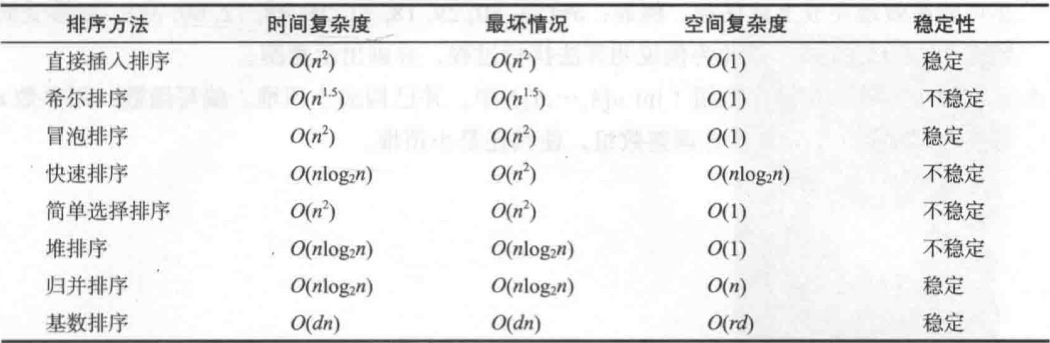
\includegraphics[width=13cm]{3.jpg}
    \caption{排序算法比较}
\end{figure}

\subsection{改进方法}

每种排序算法都是固定的,不需要改进。



\section{地铁修建}
\subsection{数据结构}
无向图、并查集
\subsection{算法设计思想}
先读入所有的边,并按权值从小到大排序。之后按权从小到大归并与边相连的两个顶点,并通过并查集检查顶点是否相连,当顶点1与顶点N连通时,当前边的权值即为最少的施工天数中最大的天数。
\subsection{源程序}
\begin{lstlisting}[caption=main.cpp,captionpos=b]
    #include <iostream>
    #include <vector>
    #include <algorithm>
    #include <string.h>
    #define NONE -1

    using namespace std;

    struct Edge{
        int v1;
        int v2;
        int weight;

        Edge(int v1In, int v2In, int weightIn): v1(v1In), v2(v2In), weight(weightIn){}

        bool operator<(const Edge& e)
        {
            return weight < e.weight;
        }
    };

    int findRoot(int fa[], int v)
    {
        if (fa[v] == NONE)
            return v;
        else
            return fa[v] = findRoot(fa, fa[v]);
    }

    int N, M;
    int main()
    {
        cin >> N >> M;
        vector<Edge> edges;

        int v1, v2, weight;
        for (int i = 1; i <= M; i++)
        {
            cin >> v1 >> v2 >> weight;
            edges.push_back(Edge(v1, v2, weight));
        }

        int father[N+1];
        memset(father, NONE, sizeof(father));//并查集初始化

        sort(edges.begin(), edges.end());//按照施工天数从小到大排序

        //模拟施工过程
        for (int i = 0; i < M; i++)
        {
            //归并两棵子树
            father[findRoot(father, edges[i].v1)] = findRoot(father, edges[i].v2);

            if (findRoot(father, 1) == findRoot(father, N))
            {
                cout << edges[i].weight;
                return 0;
            }
        }
    }

    /*
    input sample1:
    6 6
    1 2 4
    2 3 4
    3 6 7
    1 4 2
    4 5 5
    5 6 6

    output sample1:
    6

    input sample2:

    output sample2:

    input sample3:

    output sample3:

    */
\end{lstlisting}
\subsection{测试数据及其结果}
\begin{figure}[htbp] % h为当前位置,!htb为忽略美学标准,htbp为浮动图形
    \centering
    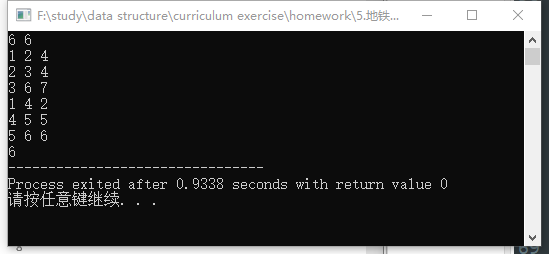
\includegraphics[width=8cm]{7.png}
    \caption{实验截图}
\end{figure}
\subsection{时间复杂度}
$$O(nlog_{2}n)$$
\subsection{改进方法}
本题有多种解法,还可以采用dijkstra算法的思想求解。


\section{社交网络图中结点的“重要性”计算}
\subsection{数据结构}
无向图
\subsection{算法设计思想}
核心为求无权图的单源最短路径,方法依旧采用BFS,然后重复n次即可。
\subsection{源程序}
\begin{lstlisting}[caption=main.cpp,captionpos=b]
    #include <iostream>
    #include <queue>
    #include <string.h>

    #define INT_MAX 0x3f3f3f3f
    #define N_MAX 1001
    #define ERROR -1.0

    using namespace std;

    void ReadIn();
    bool Calculate();
    void Print();

    bool graph[N_MAX][N_MAX];//存放该无权无向图
    double Cc[N_MAX];//紧密度中心性
    int N, M;
    int K;

    int main()
    {
        ReadIn();//读入数据

        if (!Calculate())
            memset(Cc, 0, sizeof(Cc));//若是非连通图,全设0

        Print();//输出结果
    }

    void ReadIn()
    {
        cin >> N >> M;

        for (int i = 1; i <= M; i++)
        {
            //建立无权无向图
            int v1, v2;
            cin >> v1 >> v2;
            graph[v1][v2] = true;
            graph[v2][v1] = true;
        }
    }

    //若图连通,返回start结点的紧密度中心性
    //若图不连通返回ERROR
    double BFS(int start)
    {
        queue<int> queue;
        int dist[N+1];
        memset(dist, INT_MAX, sizeof(dist));

        queue.push(start);
        dist[start] = 0;//起点

        int vertex;
        int count = 0;//统计被访问结点个数
        double sum = 0;//总的最短距离
        while (!queue.empty())
        {
            vertex = queue.front();
            queue.pop();
            count++;

            for (int i = 1; i <= N; i++)
            {
                if ((dist[i] == INT_MAX) && (graph[vertex][i])){
                    dist[i] = dist[vertex] + 1;
                    sum += (double)dist[i];
                    queue.push(i);
                }
            }
        }

        if (count < N)
            return ERROR;
        else if(count == N)
            return sum;
    }

    bool Calculate()
    {
        for (int i = 1; i <= N; i++)
        {
            double result = BFS(i);
            if (result == ERROR)
                return false;//图不连通
            else
                Cc[i] = (double)(N-1)/result;
        }

        return true;
    }

    void Print()
    {
        cin >> K;
        int vertex;
        for (int i = 1; i <= K; i++)
        {
            cin >> vertex;
            printf("Cc(%d)=%.2f\n", vertex, Cc[vertex]);
        }
    }

    /*

    //此题可直接在PTA上提交

    input sample1:
    5 8
    1 2
    1 3
    1 4
    2 3
    3 4
    4 5
    2 5
    3 5
    2 4 3

    output sample1:
    Cc(4)=0.80
    Cc(3)=1.00

    input sample2:

    output sample2:

    input sample3:

    output sample3:

    */
\end{lstlisting}
\subsection{测试数据及其结果}
\begin{figure}[htbp] % h为当前位置,!htb为忽略美学标准,htbp为浮动图形
    \centering
    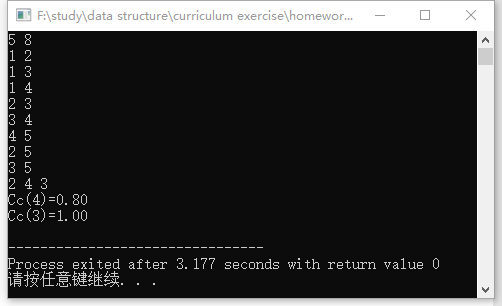
\includegraphics[width=8cm]{6.png}
    \caption{实验截图}
\end{figure}
\subsection{时间复杂度}
$$O(n^2)$$
\subsection{改进方法}
暂无改进想法。


\section{平衡二叉树操作的演示}
\subsection{数据结构}
平衡二叉排序树
\subsection{算法设计思想}

插入:
\begin{enumerate}
    \item 寻找数据插入位置。若小于当前根结点,将其递归插入至左子树,若大于,将其递归插入至右子树,若等于则插入。
    \item 向父结点回溯。若当前二叉树不平衡,回溯至最小子树并调整其至平衡。
\end{enumerate}\par

删除:
\begin{enumerate}
    \item 寻找应当删除的结点。若小于当前根结点,则在左子树中寻找,若大于,将在右子树中寻找,直至找到,执行步骤2。
    \item 若该结点为叶结点,执行步骤4。若非叶节点,执行步骤3。
    \item 若其左子树比右子树高,将该结点数据与左子树最大结点的数据交换,再删除左子树的最大结点。若右子树比左子树高同理。
    \item 删除该叶结点。
    \item 向父结点回溯。若当前二叉树不平衡,回溯至最小子树并调整其至平衡。
\end{enumerate}\par


\subsection{源程序}
\begin{lstlisting}[caption=main.cpp,captionpos=b]
    #include <iostream>
    #include <string>
    #include "avl_tree.h"

    /* run this program using the console pauser or add your own getch, system("pause") or input loop */

    int main(int argc, char** argv)
    {
        AVL_Tree avl_tree;
        const string fileName("test1.txt");
        fstream dataFile(fileName, ios::in);
        avl_tree.Create(fileName);

        //1.插入操作
        avl_tree.Insert(avl_tree.root, 9999);
        avl_tree.Insert(avl_tree.root, -9999);
        avl_tree.Insert(avl_tree.root, 2);
        avl_tree.print(avl_tree.root);
        cout << endl;

        //2.查找操作
        if (avl_tree.Find(2))
            cout << "YES" << endl;
        else
            cout << "NO" << endl;
        if (avl_tree.Find(80))
            cout << "YES" << endl;
        else
            cout << "NO" << endl;
        if (avl_tree.Find(0))
            cout << "YES" << endl;
        else
            cout << "NO" << endl;
        avl_tree.print(avl_tree.root);
        cout << endl;

        //3.删除操作
        avl_tree.Delete(avl_tree.root, 5);
        avl_tree.Delete(avl_tree.root, 0);
        avl_tree.Delete(avl_tree.root, 9999);
        avl_tree.Delete(avl_tree.root, 91);
        avl_tree.Delete(avl_tree.root, 5);
        avl_tree.Delete(avl_tree.root, 30);
        avl_tree.print(avl_tree.root);
        cout << endl;
        return 0;
    }
\end{lstlisting}
\begin{lstlisting}[caption=avl\_tree.h,captionpos=b]
    #ifndef AVL_TREE_H
    #define AVL_TREE_H

    #include <iostream>
    #include <fstream>
    #include <queue>
    #include <algorithm>
    using namespace std;

    typedef int ElemType;
    typedef struct BiNode* Position;
    typedef Position BiTree;

    struct BiNode{
        ElemType data;//关键字
        BiTree left;//左子树
        BiTree right;//右子树

        BiNode(ElemType dataIn);
    };

    class AVL_Tree{
        public:
            AVL_Tree();
            ~AVL_Tree();//销毁树

            bool Create(const string fileName);//建树
            Position Find(ElemType data);//查找值为data的结点
            Position FindMax(BiTree root);//查找以root为根的子树中,最大值结点
            Position FindMin(BiTree root);//查找以root为根的子树中,最小值结点

            Position Insert(BiTree root, ElemType data);//插入结点
            Position Delete(BiTree root);//删除子树
            Position Delete(BiTree root, ElemType data);//删除值为data的结点

            int height(BiTree root);//返回以root为根结点的树高
            Position LL_rotation(BiTree root);
            Position LR_rotation(BiTree root);
            Position RL_rotation(BiTree root);
            Position RR_rotation(BiTree root);

            void print(BiTree root);//以中序遍历方式输出结果

    //	private:
            BiTree root;//树根
    };

    //选做题 9.32
    void find_a_b(AVL_Tree& avl_tree, BiTree root, ElemType x, ElemType* a, ElemType* b);

    #endif
\end{lstlisting}
\begin{lstlisting}[caption=avl\_tree.cpp,captionpos=b]
    #include "avl_tree.h"

    BiNode::BiNode(ElemType dataIn): data(dataIn)
    {
        left = right = NULL;
    }

    AVL_Tree::AVL_Tree()
    {
        root = NULL;
    }

    AVL_Tree::~AVL_Tree()
    {
        Delete(root);
    }

    bool AVL_Tree::Create(const string fileName)
    {
        fstream dataFile(fileName, ios::in);
        if (!dataFile){
            cout << "打开文件" << fileName << "失败!" << endl;
            return false;
        }

        int data;
        while (!dataFile.eof())
        {
            dataFile >> data;
    //		cout << data << " ";//debug
            root = Insert(root, data);
        }

        dataFile.close();
        return true;
    }

    Position AVL_Tree::Find(ElemType data)
    {
        Position pos = root;
        while (pos != NULL)
        {
            if (data < pos->data)
                pos = pos->left;
            else if (data > pos->data)
                pos = pos->right;
            else
                return pos;
        }
        return NULL;
    }

    Position AVL_Tree::FindMax(BiTree root)
    {
        BiNode* p = root;
        if (p == NULL)
            return NULL;
        else
        {
            while (p->right != NULL)
            {
                p = p->right;
            }
        }
        return p;
    }

    Position AVL_Tree::FindMin(BiTree root)
    {
        BiNode* p = root;
        if (p == NULL)
            return NULL;
        else
        {
            while (p->left != NULL)
            {
                p = p->left;
            }
        }
        return p;
    }

    Position AVL_Tree::Insert(BiTree root, ElemType data)
    {
        if(root == NULL)
        {
            root = new BiNode(data);
        }
        else
        {
            if(data < root->data)
            {
                //插入到左子树
                root->left = Insert(root->left, data);
                //计算平衡因子,再判断如何旋转
                if(height(root->left) - height(root->right) == 2)
                {
                    if(data < root->left->data)
                        root = LL_rotation(root);
                    else if(data > root->left->data)
                        root = LR_rotation(root);
                }
            }
            else if(data > root->data)
            {
                //插入到右子树
                root->right = Insert(root->right, data);
                //计算平衡因子,再判断如何旋转
                if(height(root->right) - height(root->left) == 2)
                {
                    if(data > root->right->data)
                        root = RR_rotation(root);
                    else if(data < root->right->data)
                        root = RL_rotation(root);
                }
            }
        }
        return root;
    }

    Position AVL_Tree::Delete(BiTree root)
    {
        if (root != NULL){
            root->left = Delete(root->left);
            root->right = Delete(root->right);
            delete root;
            return NULL;
        }
    }

    Position AVL_Tree::Delete(BiTree root, ElemType data)
    {
        //思路:
        //1.找到结点(若不为叶结点,转化为叶结点)
        //2.删除
        //3.平衡调整
        if (root == NULL)
            return NULL;
        else
        {
            if (data < root->data) //1.找到结点
            {
                root->left = Delete(root->left, data);
            }
            else if (data > root->data) //1.找到结点
            {
                root->right = Delete(root->right, data);
            }
            else
            {
                //2.删除
                if ((root->left == NULL) && (root->right == NULL))
                {
                    delete root;
                    if (root == this->root)//特殊情况
                        this->root = NULL;
                    return NULL;
                }
                else//1.(若不为叶结点,转化为叶结点)
                {
                    Position pos;
                    if (height(root->left) > height(root->right))
                    {
                        pos = FindMax(root->left);
                        //交换data与左子树最大值
                        root->data = pos->data;
                        pos->data = data;
                        root->left = Delete(root->left, data);
                    }
                    else
                    {
                        pos = FindMin(root->right);
                        //交换data与右子树最小值
                        root->data = pos->data;
                        pos->data = data;
                        root->right = Delete(root->right, data);
                    }
                }
            }
        }

        //3.平衡调整
    //	if (height(root->left) - height(root->right) == 2)
    //	{
    //		if (height(root->left->left) >= height(root->left->right))
    //			root = LL_rotation(root);
    //		else
    //			root = LR_rotation(root);
    //	}
    //	else if (height(root->left) - height(root->right) == -2)
    //	{
    //		if (height(root->right->right) >= height(root->right->left))
    //			root = RR_rotation(root);
    //		else
    //			root = RL_rotation(root);
    //	}

        return root;
    }

    int AVL_Tree::height(BiNode* root)
    {
        if (root == NULL)
            return 0;
        else
            return 1 + max(height(root->left), height(root->right));
    }

    Position AVL_Tree::LL_rotation(BiTree root)
    {
        BiNode* p1 = root->left;
        BiNode* p2 = p1->right;
        root->left = p2;
        p1->right = root;
        return p1;
    }

    Position AVL_Tree::LR_rotation(BiTree root)
    {
        BiNode* p1 = root->left;
        BiNode* p2 = p1->right;
        root->left = p2->right;
        p2->right = root;
        p1->right = p2->left;
        p2->left = p1;
        return p2;
    }

    Position AVL_Tree::RL_rotation(BiTree root)
    {
        BiNode* p1 = root->right;
        BiNode* p2 = p1->left;
        root->right = p2->left;
        p2->left = root;
        p1->left = p2->right;
        p2->right = p1;
        return p2;
    }

    Position AVL_Tree::RR_rotation(BiTree root)
    {
        BiNode* p1 = root->right;
        BiNode* p2 = p1->left;
        root->right = p2;
        p1->left = root;
        return p1;
    }

    void AVL_Tree::print(BiTree root)
    {
        if (root == this->root)
            cout << endl << "平衡二叉树的中序遍历如下:" << endl;
        if (root == NULL)
            return;
        else if (root != NULL){
            print(root->left);
            cout << root->data << " ";
            print(root->right);
        }

    //	queue<BiNode*> queue;
    //	queue.push(root);
    //	BiNode* p;
    //	while (!queue.empty())
    //	{
    //		p = queue.front();
    //		queue.pop();
    //
    //		if (p->left != NULL)
    //			queue.push(p->left);
    //		if (p->right != NULL)
    //			queue.push(p->right);
    //
    //		cout << p->data << " 对应结点树高为:" << height(p) << endl;
    //	}
    }

    //选做题 9.32
    void find_a_b(AVL_Tree& avl_tree, BiTree root, ElemType x, ElemType* a, ElemType* b)
    {
        if (root == NULL)
            return;
        else
        {
            if (root->data < x)
            {
                *a = root->data;
                find_a_b(avl_tree, root->right, x, a, b);
            }
            else if (root->data > x)
            {
                *b = root->data;
                find_a_b(avl_tree, root->left, x, a, b);
            }
            else
            {
                Position pos1 = avl_tree.FindMax(root->left);
                Position pos2 = avl_tree.FindMin(root->right);

                if (pos1 != NULL)
                    *a = pos1->data;
                if (pos2 != NULL)
                    *b = pos2->data;
            }
        }
    }
\end{lstlisting}

\subsection{测试数据及其结果}
\begin{figure}[htbp] % h为当前位置,!htb为忽略美学标准,htbp为浮动图形
    \centering
    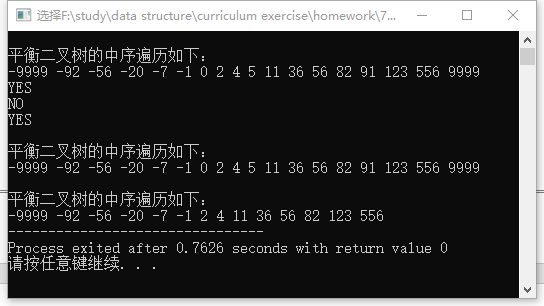
\includegraphics[width=8cm]{5.png}
    \caption{实验截图}
\end{figure}
\subsection{时间复杂度}
$$O(log_{2}n)$$
\subsection{改进方法}
将递归函数改为非递归函数,进一步加深理解。


\section{Huffman编码与解码}
\subsection{数据结构}
Huffman树
\subsection{算法设计思想}
利用最小堆建树,为每个结点编码时采用层序遍历的方式编码。为每个字符编码时只需在对应的Huffman树上查找其对应的叶结点即可。文件读写时,二进制文件中前四个字节存放数据的有效位数,第五个字节开始存放数据,解码时先读入前四字节确定数据的总位数,再进行解码。解码过程即编码逆过程。
\subsection{源程序}
\begin{lstlisting}[caption=main.cpp,captionpos=b]
    #include <iostream>
    #include "huffmantree.h"

    /* run this program using the console pauser or add your own getch, system("pause") or input loop */

    int main(int argc, char** argv)
    {
        const string sourceFile("source.txt");//未编码文件名
    //	const string sourceFile("test.txt");//测试文件

        //要求一
        CharTable charTable;
        charTable.calculateFreq(sourceFile);//统计词频
        HuffmanTree hTree(charTable);//建树
        hTree.show("Huffman.txt");//打印词频及编码,并写入文件

        //要求二
        hTree.encode(sourceFile, "code.dat");//给文件编码

        //要求三
        hTree.decode("code.dat", "解码结果.txt");//给文件解码

        return 0;
    }
\end{lstlisting}
\begin{lstlisting}[caption=huffmantree.h,captionpos=b]
    #ifndef HUFFMANTREE_H
    #define HUFFMANTREE_H

    #include <iostream>
    #include <fstream>
    #include <string>
    #include <queue>
    #include <iomanip>
    #include <string.h>
    #include <bitset>
    #include "chartable.h"

    using namespace std;

    struct BiNode{
        char data;//英文字符
        int weight;//字符权值,即其词频
        BiNode* left;
        BiNode* right;
        string codes;//编码结果

        BiNode(char c, int w);
        BiNode(int w);
        ~BiNode();

        void show();//打印词频及编码
    };

    //重写仿函数以建立最小堆
    struct cmp{
        bool operator()(BiNode* n1, BiNode* n2);
    };

    class HuffmanTree{
        public:
            HuffmanTree(CharTable& charTable);//建树
            ~HuffmanTree();//销毁Huffman tree(递归)

            void encode(const string& filename1, const string& filename2);//编码
            void decode(const string& filename1, const string& filename2);//解码

            void show(const string& filename);//打印词频及编码,并写入文件

        private:
            BiNode* root;//树根
            map<char, string> codeTable;//编码表
    };

    #endif
\end{lstlisting}
\begin{lstlisting}[caption=huffmantree.cpp,captionpos=b]
    #include "huffmantree.h"

    const int width = 25;//设置输出域宽

    bool cmp::operator()(BiNode* n1, BiNode* n2)
    {
        return n1->weight > n2->weight;
    }

    BiNode::BiNode(char c, int w): data(c), weight(w)
    {
        left = right = NULL;
    }

    BiNode::BiNode(int w): weight(w)
    {
        left = right = NULL;
    }

    BiNode::~BiNode()
    {
        if (left != NULL)
        {
            delete left;
            left = NULL;
        }
        if (right != NULL)
        {
            delete right;
            right = NULL;
        }
    }

    void BiNode::show()
    {
        cout << "char: " << data
             << setw(width) << "frequency: " << weight
             << setw(width) << "codes: " << codes
             << endl;
    }

    HuffmanTree::HuffmanTree(CharTable& charTable)
    {
        //建立最小堆
        priority_queue<BiNode*, vector<BiNode*>, cmp> minHeap;

        auto iter = charTable.table.begin();
        for (; iter != charTable.table.end(); iter++)
        {
            BiNode* p = new BiNode(iter->first, iter->second);
            minHeap.push(p);
        }

        //建树
        BiNode* min1;
        BiNode* min2;
        while (minHeap.size() != 1)
        {
            min1 = minHeap.top();
            minHeap.pop();
            min2 = minHeap.top();
            minHeap.pop();

            BiNode* root = new BiNode(min1->weight + min2->weight);
            root->left = min1;
            root->right = min2;

            minHeap.push(root);
        }

        //记录树根
        root = minHeap.top();

        //给每个结点编码(基于层序遍历)
        queue<BiNode*> queue;
        BiNode* p = root;

        if (p == NULL)
            return;

        queue.push(p);
        while (!queue.empty())
        {
            p = queue.front();
            queue.pop();

            if (p->left != NULL){
                p->left->codes = p->codes + "0";
                queue.push(p->left);
            }
            if (p->right != NULL){
                p->right->codes = p->codes + "1";
                queue.push(p->right);
            }

            //将叶结点加入编码表
            if ((p->left == NULL) && (p->right == NULL))
            {
                codeTable.insert(pair<char, string>(p->data, p->codes));
            }
        }
    }

    HuffmanTree::~HuffmanTree()
    {
        if (root != NULL)
        {
            delete root;//递归实现
            root = NULL;
        }
    }

    void HuffmanTree::show(const string& filename)
    {
        fstream file(filename.data(), ios::out);
        if (file.bad()){
            cout << "cann't open " << filename << endl;
            return;
        }

        queue<BiNode*> queue;
        BiNode* p = root;

        if (p == NULL)
            return;

        cout << "字符: "
             << setw(width) << "词频:     "
             << setw(width) << "编码:"
             << endl;
        file << "字符: "
             << setw(width) << "词频:     "
             << setw(width) << "编码:"
             << endl;

        queue.push(p);
        while (!queue.empty())
        {
            p = queue.front();
            queue.pop();

            if (p->left != NULL){
                queue.push(p->left);
            }
            if (p->right != NULL){
                queue.push(p->right);
            }

            //只对叶结点进行输出
            if ((p->left == NULL) && (p->right == NULL))
            {
                //打印
                p->show();
                //写入文件
                file << "char: " << p->data
                     << setw(width) << "frequency: " << p->weight
                     << setw(width) << "codes: " << p->codes
                     << endl;
            }
        }

        file.close();
    }

    void HuffmanTree::encode(const string& filename1, const string& filename2)
    {
        fstream sourceFile(filename1.data(), ios::in);//打开原文本文件
        if (sourceFile.bad()){
            cout << "cann't open " << filename1 << endl;
            return;
        }
        fstream desFile(filename2.data(), ios::out | ios::binary);//创建目标二进制文件
        if (desFile.bad()){
            cout << "cann't open " << filename2 << endl;
            return;
        }

        string codes;//所有编码
        //每次读入一个字符,将其编码追加入codes
        char c1;
        while (sourceFile.get(c1))//每次读入一字符
        {
            auto iter = codeTable.find(c1);
            if (iter == codeTable.end())//c1不在编码表中,报错
            {
                cout << "ERROR!!!";
                return;
            }
            else//c1在编码表中
                codes.append(iter->second);
        }

    //	cout << "codes: " << codes << endl;//debug

        //二进制文件前四个字节存放数据的有效位数
        int bitSize = codes.size();
        desFile.write((const char*)(&bitSize), sizeof(bitSize));

        //第五个字节开始存放数据
        int byteSize = codes.size()/8 + 1;

        for (int i = 0; i < byteSize; i++)
        {
            bitset<8> byte(codes.substr(i*8, 8));//直接用string初始化byte

            //将一字节编码写入文件
            desFile.write((const char*)&byte, byte.size()/8);
        }

        sourceFile.close();
        desFile.close();
    }

    void HuffmanTree::decode(const string& filename1, const string& filename2)
    {
        fstream sourceFile(filename1.data(), ios::in | ios::binary);//打开原二进制文件
        if (sourceFile.bad()){
            cout << "cann't open " << filename1 << endl;
            return;
        }
        fstream desFile(filename2.data(), ios::out);//创建目标文本文件
        if (desFile.bad()){
            cout << "cann't open " << filename2 << endl;
            return;
        }

        //先读入前四字节
        int bitSize;
        sourceFile.read((char*)(&bitSize), sizeof(bitSize));
        int byteSize = bitSize/8 + 1;

        string codes;
        for (int i = 0; i < byteSize; i++)
        {
            //读入一字节
            bitset<8> byte;
            sourceFile.read((char*)&byte, byte.size()/8);
            //将这一字节编码转为string
            codes.append(byte.to_string());
        }

        //先将最后八位全部读入,再删去冗余部分
        int n = byteSize*8 - bitSize;
        cout << "n: " << n << endl;//debug
        codes.erase((byteSize-1)*8, n);

    //	cout << "codes: " << codes << endl;//debug
    //	return;

        string curCodes;
        char c;
        BiNode* p;
        int i = 0;
        while (i < codes.size())
        {
            curCodes.clear();//先清空上次的编码

            while (1)//一次循环解码一字符
            {
                if (i >= codes.size())//表明编码结束
                    break;

                curCodes += codes.at(i++);
                p = root;
                int pos = 0;

                //寻找curCodes对应的叶结点
                while ((p != NULL) && (pos < curCodes.size()))
                {
                    if (curCodes.at(pos) == '0')
                        p = p->left;
                    else if (curCodes.at(pos) == '1')
                        p = p->right;
                    pos++;
                }

                //若p指向叶结点且pos指向curCodes末尾,则可解码一个字符
                if ((p->left == NULL) && (p->right == NULL) &&
                    (pos == curCodes.size()))
                {
                    break;
                }
                //反之,需要继续读入二进制码
            }

            desFile << p->data;//成功解码一个字符
        }

        sourceFile.close();
        desFile.close();
    }
\end{lstlisting}
\begin{lstlisting}[caption=chartable.h,captionpos=b]
    #ifndef CHARTABLE_H
    #define CHARTABLE_H

    #include <string>
    #include <map>

    using namespace std;

    class CharTable{
        public:
            //计算文件中所有出现字符的词频
            void calculateFreq(const string& filename);

        private:
            //存放词频
            map<char, int> table;

        friend class HuffmanTree;
    };

    #endif
\end{lstlisting}
\begin{lstlisting}[caption=chartable.cpp,captionpos=b]
    #include "chartable.h"

    #include <iostream>
    #include <fstream>

    void CharTable::calculateFreq(const string& filename)
    {
        fstream file(filename.data());
        if (file.bad()){
            cout << "cann't open " << filename << endl;
            return;
        }

        //每次读入一个字符
        //若不在表中,将其插入表中
        //若在表中,其词频加1
        char c1;
        while (file.get(c1))//每次读入一字符
        {
            auto iter = table.find(c1);
            if (iter == table.end())//c1不在表中
            {
                table.insert(pair<char, int>(c1, 1));
            }
            else//c1在表中
            {
                iter->second++;
            }
        }

        file.close();
    }
\end{lstlisting}
\subsection{测试数据及其结果}
\begin{figure}[htbp] % h为当前位置,!htb为忽略美学标准,htbp为浮动图形
    \centering
    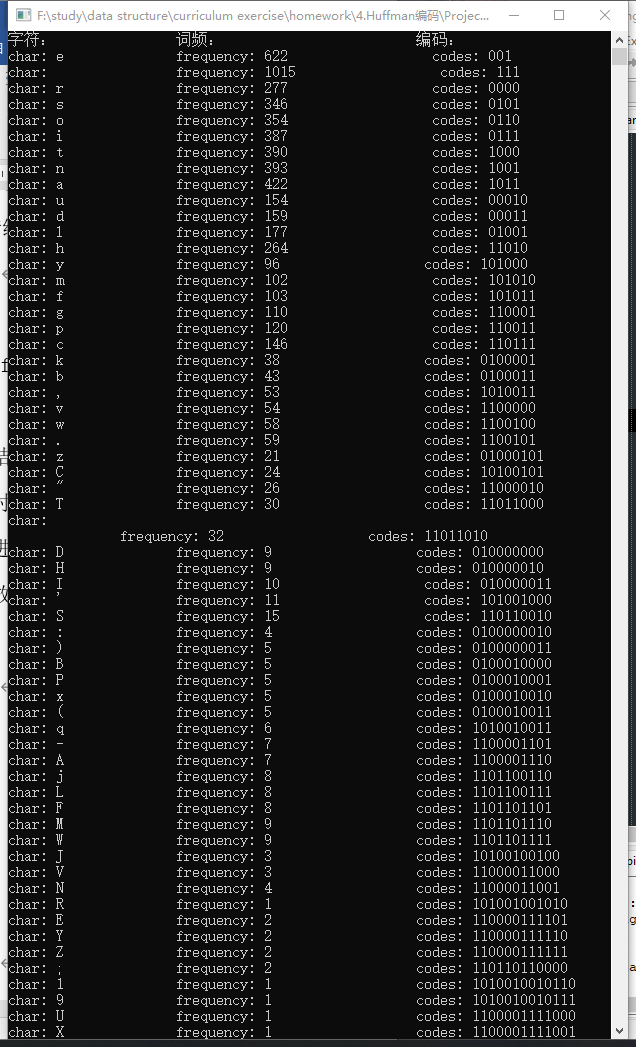
\includegraphics[width=8cm]{4.png}
    \caption{实验截图}
\end{figure}
\newpage
\subsection{时间复杂度}
$$O(n)$$

\subsection{改进方法}
采用其他编码方法如LZW编码。

\section{家谱管理系统}
\subsection{数据结构}
树
\subsection{算法设计思想}
将祖先结点作为家族类的成员变量,每一个结点记录一对夫妻的信息,以及存放后代夫妻结点的数组。
\subsection{源程序}
\begin{lstlisting}[caption=main.cpp,captionpos=b]
    #include <iostream>
    #include "familytree.h"

    /* run this program using the console pauser or add your own getch, system("pause") or input loop */

    int main(int argc, char** argv)
    {
        const string fileName("data.txt");//原始数据文件
    //	const string fileName("test.txt");

        familyTree family(fileName);

        int x;
        while(1)
        {
    //		system("cls");

            cout << "请输入数字实现相应功能噢。" << endl
                 << "若想显示家谱所有人信息,请按1" << endl
                 << "若想显示第n 代所有人的信息,请按2" << endl
                 << "若想显示某人的信息,请按3" << endl
                 << "若想查询两人之间关系,请按4" << endl
                 << "若想为某夫妇添加孩子,请按5" << endl
                 << "若想为某人添加配偶,请按6" << endl
                 << "若想删除某成员,请按7" << endl
                 << "若想修改某成员信息,请按8" << endl
                 << "若想按照出生/死亡日期查询成员信息,请按9" << endl
                 << "若想退出程序,请按0" << endl << endl
                 << "请输入:";
            cin >> x;
            cout << endl;
            Operation(x, family);//执行相应操作

            system("pause");
        }
    }
\end{lstlisting}
\begin{lstlisting}[caption=familytree.h,captionpos=b]
    #ifndef FAMILYTREE_H
    #define FAMILYTREE_H

    #include <iostream>
    #include <fstream>
    #include <vector>
    #include <queue>
    #include <string>
    #include <string.h>
    #include <algorithm>
    #define NONE -1
    using namespace std;

    struct Person{
        string name;//姓名
        bool gender;//性别
        bool married;//婚否
        bool alive;//健在否
        string date;//出生/死亡日期
        string address;//住址

        Person();
        Person(string& nameIn, bool genderIn, bool marriedIn, bool aliveIn, string& dateIn, string& addressIn);
    };

    struct Couple{
    //	bool which;//若真,husband为子,若假,wife为女
        Person husband;
        Person wife;
        int generation;//第几代人

        vector<Couple> offspring;//后代

        Couple();
        Couple(Person husbandIn, Person wifeIn, int geIn = NONE);
    };

    class familyTree{
        public:
            familyTree(const string& fileName);//读取数据并建树
            ~familyTree();//销毁树

            void show();//显示所有人信息
            void show(int generation);//显示第n代所有人信息
            void show(const Person& person, bool familyMember = false);//显示此人信息
            void show(bool alive, const string& date);//按出生/死亡日期显示信息
            void showRelation(const string& name1, const string& name2);//显示两人关系

            Couple* find(const string& name);//按姓名查找
            Couple* findParents(const string& name);//返回其双亲

            void addCouple(const string& name, const Person person);//添加配偶
            void addChild(const string& name, Couple couple);//添加孩子
            void deletePerson(const string& name);//删除成员
            void modify(const string& name, Person person);//修改成员信息

    //	private:
            Couple ancestor;//根结点

            int personCnt;//总人数
    };

    void Operation(int x, familyTree& family);
    void operation0();//退出程序
    void operation1(familyTree& family);//显示家谱所有人信息
    void operation2(familyTree& family);//显示第n 代所有人的信息
    void operation3(familyTree& family);//显示某人的信息
    void operation4(familyTree& family);//查询两人之间关系
    void operation5(familyTree& family);//为某夫妇添加孩子
    void operation6(familyTree& family);//为某人添加配偶
    void operation7(familyTree& family);//删除某成员
    void operation8(familyTree& family);//修改某成员信息
    void operation9(familyTree& family);//按照出生/死亡日期查询成员信息

    #endif
\end{lstlisting}
\begin{lstlisting}[caption=familytree.cpp,captionpos=b]
    #include "familytree.h"

    Person::Person(){}

    Person::Person(string& nameIn, bool genderIn, bool marriedIn, bool aliveIn, string& dateIn, string& addressIn)
                  :name(nameIn), gender(genderIn), married(marriedIn), alive(aliveIn), date(dateIn), address(addressIn)
    {

    }

    Couple::Couple(){}

    Couple::Couple(Person husbandIn, Person wifeIn, int geIn)
                  : husband(husbandIn), wife(wifeIn), generation(geIn)
    {

    }

    familyTree::familyTree(const string& fileName)
    {
        personCnt = 0;
        fstream dataFile(fileName, ios::in);

        string name1, name2, date, address, tmp1, tmp2, tmp3;
        bool gender, married, alive;
        char x;
        while (dataFile.get(x))
        {
            if (personCnt != 0)
                dataFile >> name1;

            dataFile >> name2 >> tmp1 >> tmp2 >> tmp3 >> date >> address;
            dataFile.ignore();//读掉换行符

            if (tmp1 == "男")				gender = true;
            else if (tmp1 == "女")			gender = false;
            if (tmp2 == "已婚")				married = true;
            else if (tmp2 == "未婚")		married = false;
            if (tmp3 == "健在")				alive = true;
            else if (tmp3 == "已故")		alive = false;
            Person person(name2, gender, married, alive, date, address);

            if (x == '5')//添加孩子
            {
                if (gender)
                    addChild(name1, Couple(person, Person()));
                else
                    addChild(name1, Couple(Person(), person));
            }
            else if (x == '6')//添加配偶
            {
                addCouple(name1, person);
            }
        }

        dataFile.close();
    }

    familyTree::~familyTree(){}

    //显示所有人信息(层序遍历)
    void familyTree::show()
    {
        cout << "以下是家谱中所有人的信息:" << endl;

        queue<Couple*> Queue;
        Queue.push(&ancestor);

        while (!Queue.empty())
        {
            Couple* cpl = Queue.front();
            Queue.pop();

            //输出夫妇信息
            show(cpl->husband);
            show(cpl->wife);

            for (int i = 0; i < cpl->offspring.size(); i++)
                Queue.push(&cpl->offspring.at(i));
        }
    }

    //显示第n代所有人信息 (层序遍历)
    void familyTree::show(int generation)
    {
        cout << "以下是第 " << generation << " 代所有人的信息:" << endl;

        queue<Couple*> Queue;
        Queue.push(&ancestor);
    //	Couple* lastPtr = Queue.front();//指向每层最后一个结点
    //	int level = 1;

        while (!Queue.empty())
        {
            Couple* cpl = Queue.front();
            Queue.pop();

            //输出夫妇信息
            if (cpl->generation == generation)
            {
                show(cpl->husband);
                show(cpl->wife);
            }
            else if (cpl->generation > generation)
                return;

            for (int i = 0; i < cpl->offspring.size(); i++)
                Queue.push(&cpl->offspring.at(i));

    //		if (cpl == lastPtr)
    //		{
    //			lastPtr = Queue.back();
    //			level++;
    //		}
        }
    }

    //显示此人信息
    void familyTree::show(const Person& person, bool familyMember)
    {
        if (person.name.empty())
            return;
    //	cout << "here4" << endl;//debug

        cout << "以下为 " << person.name << " 的全部信息:" << endl
             << person.name << " ";
        if (person.gender)		cout << "男 ";
        else				cout << "女 ";
        if (person.married)		cout << "已婚 ";
        else				cout << "未婚 ";
        if (person.alive)		cout << "健在 ";
        else				cout << "已故 ";
        cout << person.date << " " << person.address << endl << endl;

        if (familyMember)
        {
            Couple* cpl = findParents(person.name);//找到其双亲
            if (cpl != NULL)
            {
                cout << "以下为 " << person.name << " 双亲的全部信息:" << endl << endl;
                show(cpl->husband);
                show(cpl->wife);
            }
            else
                cout << "未找到 " << person.name << " 的双亲。" << endl << endl;

            cpl = find(person.name);//找到其本人
            if (cpl == NULL)
                cout << "未找到 " << person.name << ",请检查输入是否合法。" << endl << endl;
            else if (cpl->offspring.size() == 0)
                cout << person.name << " 无子女。" << endl << endl;
            else
            {
                cout << "以下为 " << person.name << " 子女的全部信息:" << endl << endl;
                for (int i = 0; i < cpl->offspring.size(); i++)
                {
                    show(cpl->offspring[i].husband);
                    show(cpl->offspring[i].wife);
                }
            }
        }
    }

    //显示两人关系
    void familyTree::showRelation(const string& name1, const string& name2)
    {
        if (name1 == name2)
        {
            cout << "这是同一人。" << endl;
            return;
        }

        Couple* cpl1 = find(name1);
        Couple* cpl2 = find(name2);
        if (cpl1 == cpl2)
        {
            cout << name1 << "与 "  << name2 << " 是夫妻关系。" << endl;
            return;
        }

        int ge1 = cpl1->generation;
        int ge2 = cpl2->generation;
        int minG = min(ge1, ge2);
        Couple* cpl;

        if (ge1 > minG)
        {
            string tmp = name1;

            cout << name1 << " ";
            while (ge1-- > minG)
            {
                cout << "的父亲";
                cpl = findParents(tmp);
                tmp = cpl->husband.name;
            }

            if (cpl->husband.name == name2)
                cout << "是 " << name2 << endl;
            else if (cpl->wife.name == name2)
                cout << "的妻子是 " << name2 << endl;
            else
                cout << "与 "  << name2 << " 是兄弟姐妹关系。" << endl;
        }
        else if (ge2 > minG)
        {
            string tmp = name2;
            cout << name2 << " ";
            while (ge2-- > minG)
            {
                cout << "的父亲";
                cpl = findParents(tmp);
                tmp = cpl->husband.name;
            }

            if (cpl->husband.name == name1)
                cout << "是 " << name1 << endl;
            else if (cpl->wife.name == name1)
                cout << "的妻子是 " << name1 << endl;
            else
                cout << "与 "  << name1 << " 是兄弟姐妹关系。" << endl;
        }
        else
            cout << name1 << "与 "  << name2 << " 是兄弟姐妹关系。" << endl;
    }

    //按姓名查找(层序遍历)
    Couple* familyTree::find(const string& name)
    {
        queue<Couple*> Queue;
        Queue.push(&ancestor);

        while (!Queue.empty())
        {
            Couple* cpl = Queue.front();
            Queue.pop();

            if ((cpl->husband.name == name) || (cpl->wife.name == name))//找到
                return cpl;

            for (int i = 0; i < cpl->offspring.size(); i++)
                Queue.push(&cpl->offspring.at(i));
        }
        //未找到
        return NULL;
    }

    //返回其双亲(层序遍历)
    Couple* familyTree::findParents(const string& name)
    {
        queue<Couple*> Queue;
        Queue.push(&ancestor);

        while (!Queue.empty())
        {
            Couple* cpl = Queue.front();
            Queue.pop();

            for (int i = 0; i < cpl->offspring.size(); i++)
                if ((cpl->offspring[i].husband.name == name) || (cpl->offspring[i].wife.name == name))//找到
                    return cpl;

            for (int i = 0; i < cpl->offspring.size(); i++)
                Queue.push(&cpl->offspring.at(i));
        }
        //未找到
        return NULL;
    }

    //按出生/死亡日期查找(层序遍历)
    void familyTree::show(bool alive, const string& date)
    {
        cout << "以下为符合要求的所有成员信息:" << endl;
        queue<Couple*> Queue;
        Queue.push(&ancestor);

        while (!Queue.empty())
        {
            Couple* cpl = Queue.front();
            Queue.pop();

            if ((cpl->husband.alive == alive) && (cpl->husband.date == date))
                show(cpl->husband);
            if ((cpl->wife.alive == alive) && (cpl->wife.date == date))
                show(cpl->wife);

            for (int i = 0; i < cpl->offspring.size(); i++)
                Queue.push(&cpl->offspring.at(i));
        }
    }

    //添加孩子
    void familyTree::addChild(const string& name, Couple couple)
    {
        if (personCnt == 0)
        {
            ancestor = couple;
            ancestor.generation = 1;
        }
        else
        {
            Couple* cpl = find(name);
            if (cpl == NULL)
            {
                cout << "未找到 " << name << ",请检查输入是否合法。" << endl << endl;
                return;
            }
            couple.generation = cpl->generation+1;
            cpl->offspring.push_back(couple);
        }
        personCnt++;
    }

    //添加配偶
    void familyTree::addCouple(const string& name, const Person person)
    {
    //	cout << "here5" << endl;//debug
        Couple* cpl = find(name);
        if (cpl->husband.name == name)
            cpl->wife = person;
        else
            cpl->husband = person;
        personCnt++;
    }

    //删除成员
    void familyTree::deletePerson(const string& name)
    {
        if ((ancestor.husband.name == name) || (ancestor.wife.name == name))
            ancestor.~Couple();
        else
        {
            Couple* cpl = findParents(name);
            if (cpl == NULL)
            {
                cout << "未找到 " << name << ",请检查输入是否合法。" << endl << endl;
                return;
            }
            auto iter = cpl->offspring.begin();
            for (; iter != cpl->offspring.end(); )
                if ((iter->husband.name == name) || (iter->wife.name == name))
                {
                    iter = cpl->offspring.erase(iter);
                }
                else
                    iter++;
        }
    }

    //修改成员信息
    void familyTree::modify(const string& name, Person person)
    {
        Couple* cpl = find(name);
        if (cpl->husband.name == name)
            cpl->husband = person;
        else if (cpl->wife.name == name)
            cpl->wife = person;
    }

    void Operation(int x, familyTree& family)
    {
        switch (x)
        {
            case 0: operation0();break;
            case 1: operation1(family);break;
            case 2: operation2(family);break;
            case 3: operation3(family);break;
            case 4: operation4(family);break;
            case 5: operation5(family);break;
            case 6: operation6(family);break;
            case 7: operation7(family);break;
            case 8: operation8(family);break;
            case 9: operation9(family);break;
            default :operation0();break;
        }
    }

    void operation0()
    {
        cout<< "程序已退出。" << endl;
        exit(0);
    }

    void operation1(familyTree& family)
    {
        family.show();
    }

    void operation2(familyTree& family)
    {
        int generation;
        cout << "您想显示第几代人的信息呢?" << endl;
        cin >> generation;
        family.show(generation);
    }

    void operation3(familyTree& family)
    {
        string name;
        cout << "您想显示谁的信息呢?" << endl;
        cin >> name;
        bool familyMember;
        cout << "您想显示 " << name << " 家庭成员的信息吗?若想输入1,反之输入0:" << endl;
        cin >> familyMember;
        Couple* cpl = family.find(name);
        if (cpl == NULL)
        {
            cout << "未找到 " << name << ",请检查输入是否合法。" << endl << endl;
            return;
        }
        else if (cpl->husband.name == name)
            family.show(cpl->husband, familyMember);
        else
            family.show(cpl->wife, familyMember);
    }

    void operation4(familyTree& family)
    {
        string name1, name2;
        cout << "您想查询谁与谁之间的信息呢?" << endl;
        cin >> name1 >> name2;
        family.showRelation(name1, name2);
    }

    void operation5(familyTree& family)
    {
        string name1, name2, date, address, tmp1, tmp2, tmp3;
        bool gender, married, alive;

        cout << "您想为谁添加孩子呢?" << endl;
        cin >> name1;
        cout << "请输入此人所有信息:" << endl;
        cin >> name2 >> tmp1 >> tmp2 >> tmp3 >> date >> address;

        if (tmp1 == "男")				gender = true;
        else if (tmp1 == "女")			gender = false;
        if (tmp2 == "已婚")				married = true;
        else if (tmp2 == "未婚")		married = false;
        if (tmp3 == "健在")				alive = true;
        else if (tmp3 == "已故")		alive = false;
        Person person(name2, gender, married, alive, date, address);

        if (gender)
            family.addChild(name1, Couple(person, Person()));
        else
            family.addChild(name1, Couple(Person(), person));
    }

    void operation6(familyTree& family)
    {
        string name1, name2, date, address, tmp1, tmp2, tmp3;
        bool gender, married, alive;

        cout << "您想为谁添加配偶呢?" << endl;
        cin >> name1;
        cout << "请输入此人所有信息:" << endl;
        cin >> name2 >> tmp1 >> tmp2 >> tmp3 >> date >> address;

        if (tmp1 == "男")				gender = true;
        else if (tmp1 == "女")			gender = false;
        if (tmp2 == "已婚")				married = true;
        else if (tmp2 == "未婚")		married = false;
        if (tmp3 == "健在")				alive = true;
        else if (tmp3 == "已故")		alive = false;
        Person person(name2, gender, married, alive, date, address);

        family.addCouple(name1, person);
    }

    void operation7(familyTree& family)
    {
        string name;
        cout << "您想删除哪位成员呢?" << endl;
        cin >> name;

        family.deletePerson(name);
    }

    void operation8(familyTree& family)
    {
        string name1, name2, date, address, tmp1, tmp2, tmp3;
        bool gender, married, alive;

        cout << "您想修改哪位成员的信息呢?" << endl;
        cin >> name1;
        cout << "请输入此人所有信息:" << endl;
        cin >> name2 >> tmp1 >> tmp2 >> tmp3 >> date >> address;

        if (tmp1 == "男")				gender = true;
        else if (tmp1 == "女")			gender = false;
        if (tmp2 == "已婚")				married = true;
        else if (tmp2 == "未婚")		married = false;
        if (tmp3 == "健在")				alive = true;
        else if (tmp3 == "已故")		alive = false;
        Person person(name2, gender, married, alive, date, address);

        family.modify(name1, person);
    }

    void operation9(familyTree& family)
    {
        bool alive;
        cout << "此人是否健在,若是输入1,反之输入0:" << endl;
        cin >> alive;
        string date;
        cout << "请输入出生/死亡日期:" << endl;
        cin >> date;

        family.show(alive, date);
    }
\end{lstlisting}
\subsection{测试数据及其结果}
\begin{lstlisting}[caption=,captionpos=b]
请输入数字实现相应功能噢。
若想显示家谱所有人信息,请按1
若想显示第n 代所有人的信息,请按2
若想显示某人的信息,请按3
若想查询两人之间关系,请按4
若想为某夫妇添加孩子,请按5
若想为某人添加配偶,请按6
若想删除某成员,请按7
若想修改某成员信息,请按8
若想按照出生/死亡日期查询成员信息,请按9
若想退出程序,请按0

请输入:2

您想显示第几代人的信息呢?
3
以下是第 3 代所有人的信息:
以下为 颜俊哲 的全部信息:
颜俊哲 男 已婚 健在 1976 江苏省姜堰市

以下为 申润青 的全部信息:
申润青 女 已婚 健在 1978 江苏省姜堰市

以下为 颜俊平 的全部信息:
颜俊平 男 已婚 健在 1979 北京市

以下为 朱榕 的全部信息:
朱榕 女 已婚 健在 1981 北京市

以下为 颜俊臣 的全部信息:
颜俊臣 男 已婚 健在 1982 江苏省兴化市

以下为 吴晓艳 的全部信息:
吴晓艳 女 已婚 健在 1984 江苏省兴化市

以下为 范宏奇 的全部信息:
范宏奇 男 已婚 健在 1982 天津市

以下为 颜俊卿 的全部信息:
颜俊卿 女 已婚 健在 1984 天津市

以下为 张赟 的全部信息:
张赟 男 已婚 健在 1985 天津市

以下为 赵玉冰 的全部信息:
赵玉冰 女 已婚 健在 1986 天津市

以下为 丁建华 的全部信息:
丁建华 男 已婚 健在 1982 江苏省兴化市

以下为 颜俊嫣 的全部信息:
颜俊嫣 女 已婚 健在 1985 江苏省兴化市

以下为 颜俊浩 的全部信息:
颜俊浩 男 已婚 健在 1986 北京市

以下为 孙文静 的全部信息:
孙文静 女 已婚 健在 1987 北京市

以下为 颜珺圻 的全部信息:
颜珺圻 女 未婚 健在 1996 北京市

以下为 郭恩义 的全部信息:
郭恩义 男 未婚 健在 1999 福建省厦门市

以下为 颜宇明 的全部信息:
颜宇明 男 未婚 健在 2001 江苏省南京市

以下为 颜俊曜 的全部信息:
颜俊曜 男 未婚 健在 2017 江苏省泰州市
\end{lstlisting}
\subsection{时间复杂度}
$$O(logn)$$
\subsection{改进方法}

可在界面设计上加以优化,力争用图形方式显示家族树。另外由于中国的亲缘关系错综复杂,在查询两个人关系的算法方面也有很大的改进空间。

\section{总结}
\subsection{代码行数}
\begin{table}[htbp]
    \centering
  \begin{tabular*}{0.75\textwidth}{@{\extracolsep{\fill}}lcc}
      \toprule
      题目          &行数         \\
      \midrule
      区块链         &283     \\
      迷宫问题       &388     \\
      JSON查找      &369    \\
      公交线路提示      &253    \\
      Hash表应用      &    \\
      排序算法比较      &253    \\
      地铁修建      &60    \\
      社交网络图中结点的“重要性”计算      &103    \\
      平衡二叉树操作的演示      &413    \\
      Huffman编码与解码      &417    \\
      家谱管理系统      &621    \\
      \bottomrule
  \end{tabular*}
  \end{table}
\begin{lstlisting}[caption=,captionpos=b]
总代码行数为:3160.
\end{lstlisting}
\subsection{心得体会}

总体来说,本次课设难度较大,任务量也很大,但完成之后也收获满满。\par
我总共完成了六个个必做题,五个选做题,这些选做题分别为7题、10题、18题、19题、20题,选做题分值总计12分,并且充分完成了每个题目及其要求的所有功能。\par
开始时,感觉必做题难度较大,因为每个题都会或多或少涉及一些课外的操作或技巧,比如第一题中如何获取系统进程、第四题中二进制文件按位读写、第五题中并查集的实现、第七题中平衡二叉排序树的删除操作等等,但通过与同学交流,探讨方法,以及在CSDN上参考其他博主的方法,这些问题最终都一一解决。\par
这次课设充分巩固了我在理论课上的所学知识,并得以实践。相比上机题,课设的很多题都更具有一定的实际意义,比如Huffman编码这道题,若真正实现将其按位存储,能够将文件压缩存储,又比如公交线路提示,利用真实南京公交线路图建立图的存储结构,并给出提示,充分说明了图结构的广泛应用价值。\par
这次课设也拓宽了我的知识面,学习到了很多实用的操作与技巧,在解决一个个问题的过程中也极大地锻炼了我的自学能力与知识迁移能力。\par
同时做题过程中当然免不了会有各种奇奇怪怪的bug,在给自己以及给同学调代码的过程中,自己的debug能力也有了进一步的提升。\par
总之这次课设虽然过程曲折艰辛,但完成之后还是很有成就感的。\par

\setlength{\parskip}{6pt}  %定义段间距
\vspace{4cm}
\end{document}
